% Options for packages loaded elsewhere
% Options for packages loaded elsewhere
\PassOptionsToPackage{unicode}{hyperref}
\PassOptionsToPackage{hyphens}{url}
\PassOptionsToPackage{dvipsnames,svgnames,x11names}{xcolor}
%
\documentclass[
  11pt,
  a4paper,
]{article}
\usepackage{xcolor}
\usepackage[margin=25mm]{geometry}
\usepackage{amsmath,amssymb}
\setcounter{secnumdepth}{3}
\usepackage{iftex}
\ifPDFTeX
  \usepackage[T1]{fontenc}
  \usepackage[utf8]{inputenc}
  \usepackage{textcomp} % provide euro and other symbols
\else % if luatex or xetex
  \usepackage{unicode-math} % this also loads fontspec
  \defaultfontfeatures{Scale=MatchLowercase}
  \defaultfontfeatures[\rmfamily]{Ligatures=TeX,Scale=1}
\fi
\usepackage{lmodern}
\ifPDFTeX\else
  % xetex/luatex font selection
\fi
% Use upquote if available, for straight quotes in verbatim environments
\IfFileExists{upquote.sty}{\usepackage{upquote}}{}
\IfFileExists{microtype.sty}{% use microtype if available
  \usepackage[]{microtype}
  \UseMicrotypeSet[protrusion]{basicmath} % disable protrusion for tt fonts
}{}
\makeatletter
\@ifundefined{KOMAClassName}{% if non-KOMA class
  \IfFileExists{parskip.sty}{%
    \usepackage{parskip}
  }{% else
    \setlength{\parindent}{0pt}
    \setlength{\parskip}{6pt plus 2pt minus 1pt}}
}{% if KOMA class
  \KOMAoptions{parskip=half}}
\makeatother
% Make \paragraph and \subparagraph free-standing
\makeatletter
\ifx\paragraph\undefined\else
  \let\oldparagraph\paragraph
  \renewcommand{\paragraph}{
    \@ifstar
      \xxxParagraphStar
      \xxxParagraphNoStar
  }
  \newcommand{\xxxParagraphStar}[1]{\oldparagraph*{#1}\mbox{}}
  \newcommand{\xxxParagraphNoStar}[1]{\oldparagraph{#1}\mbox{}}
\fi
\ifx\subparagraph\undefined\else
  \let\oldsubparagraph\subparagraph
  \renewcommand{\subparagraph}{
    \@ifstar
      \xxxSubParagraphStar
      \xxxSubParagraphNoStar
  }
  \newcommand{\xxxSubParagraphStar}[1]{\oldsubparagraph*{#1}\mbox{}}
  \newcommand{\xxxSubParagraphNoStar}[1]{\oldsubparagraph{#1}\mbox{}}
\fi
\makeatother


\usepackage{longtable,booktabs,array}
\newcounter{none} % for unnumbered tables
\usepackage{calc} % for calculating minipage widths
% Correct order of tables after \paragraph or \subparagraph
\usepackage{etoolbox}
\makeatletter
\patchcmd\longtable{\par}{\if@noskipsec\mbox{}\fi\par}{}{}
\makeatother
% Allow footnotes in longtable head/foot
\IfFileExists{footnotehyper.sty}{\usepackage{footnotehyper}}{\usepackage{footnote}}
\makesavenoteenv{longtable}
\usepackage{graphicx}
\makeatletter
\newsavebox\pandoc@box
\newcommand*\pandocbounded[1]{% scales image to fit in text height/width
  \sbox\pandoc@box{#1}%
  \Gscale@div\@tempa{\textheight}{\dimexpr\ht\pandoc@box+\dp\pandoc@box\relax}%
  \Gscale@div\@tempb{\linewidth}{\wd\pandoc@box}%
  \ifdim\@tempb\p@<\@tempa\p@\let\@tempa\@tempb\fi% select the smaller of both
  \ifdim\@tempa\p@<\p@\scalebox{\@tempa}{\usebox\pandoc@box}%
  \else\usebox{\pandoc@box}%
  \fi%
}
% Set default figure placement to htbp
\def\fps@figure{htbp}
\makeatother





\setlength{\emergencystretch}{3em} % prevent overfull lines

\providecommand{\tightlist}{%
  \setlength{\itemsep}{0pt}\setlength{\parskip}{0pt}}



 


\usepackage{booktabs}
\usepackage{longtable}
\usepackage{array}
\usepackage{multirow}
\usepackage{wrapfig}
\usepackage{float}
\usepackage{colortbl}
\usepackage{pdflscape}
\usepackage{tabu}
\usepackage{threeparttable}
\usepackage{threeparttablex}
\usepackage[normalem]{ulem}
\usepackage{makecell}
\usepackage{xcolor}
\renewcommand{\baselinestretch}{1.1}
\usepackage{microtype}
\frenchspacing
\usepackage{graphicx}
\usepackage{xcolor}
\usepackage{amsmath,amssymb}
\usepackage{booktabs}
\usepackage{longtable}
\usepackage{array}
\usepackage{multirow}
\usepackage{makecell}
\usepackage{pdflscape}
\usepackage{float}
\usepackage{fancyhdr}
\makeatletter
\@ifpackageloaded{caption}{}{\usepackage{caption}}
\AtBeginDocument{%
\ifdefined\contentsname
  \renewcommand*\contentsname{Table of contents}
\else
  \newcommand\contentsname{Table of contents}
\fi
\ifdefined\listfigurename
  \renewcommand*\listfigurename{List of Figures}
\else
  \newcommand\listfigurename{List of Figures}
\fi
\ifdefined\listtablename
  \renewcommand*\listtablename{List of Tables}
\else
  \newcommand\listtablename{List of Tables}
\fi
\ifdefined\figurename
  \renewcommand*\figurename{Figure}
\else
  \newcommand\figurename{Figure}
\fi
\ifdefined\tablename
  \renewcommand*\tablename{Table}
\else
  \newcommand\tablename{Table}
\fi
}
\@ifpackageloaded{float}{}{\usepackage{float}}
\floatstyle{ruled}
\@ifundefined{c@chapter}{\newfloat{codelisting}{h}{lop}}{\newfloat{codelisting}{h}{lop}[chapter]}
\floatname{codelisting}{Listing}
\newcommand*\listoflistings{\listof{codelisting}{List of Listings}}
\makeatother
\makeatletter
\makeatother
\makeatletter
\@ifpackageloaded{caption}{}{\usepackage{caption}}
\@ifpackageloaded{subcaption}{}{\usepackage{subcaption}}
\makeatother
\usepackage{bookmark}
\IfFileExists{xurl.sty}{\usepackage{xurl}}{} % add URL line breaks if available
\urlstyle{same}
\hypersetup{
  pdftitle={Decomposition of Concentration-Index Trees},
  pdfauthor={Moses Mburu},
  colorlinks=true,
  linkcolor={blue},
  filecolor={Maroon},
  citecolor={Blue},
  urlcolor={Blue},
  pdfcreator={LaTeX via pandoc}}


\title{Decomposition of Concentration-Index Trees}
\author{Moses Mburu}
\date{}
\begin{document}
\maketitle


\section{Results}\label{results}

\subsection{Exploratory Data Analysis}\label{exploratory-data-analysis}

From the exploratory analysis, we see a high under-five mortality rate
of 10.32\% (Figure~\ref{fig-results-wealth-distribution}). This was not
evenly distributed among subgroups. Among children who died before age
five, 51.3\% were from low-wealth households, compared with 42.8\% among
children alive at age five; 65.6\% had no skilled birth attendance,
compared with 56.8\% among those alive; 69.3\% were from rural areas,
compared with 60.7\% among those alive; and 67.5\% had mothers with no
education, compared with 55.2\% among those alive
(Table~\ref{tbl-appendix-weighted-baseline}). The province distribution
also shows that mortality was not evenly distributed across the DRC
provinces, with the highest under-five mortality rate observed in
Katanga (14.2\%) and the lowest in Kinshasa (6.2\%)
(Figure~\ref{fig-appendix-province-mortality-distribution}).

\begin{figure}[H]

\centering{

\pandocbounded{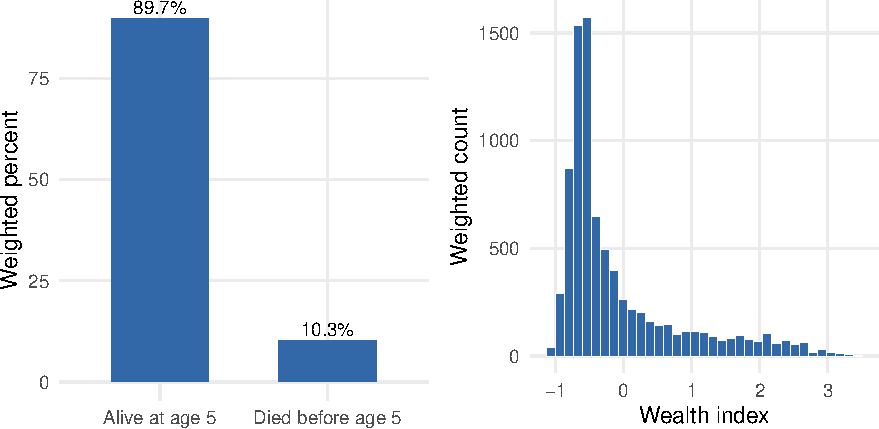
\includegraphics[keepaspectratio]{Decomposition_of_CI_Trees_MM_files/figure-pdf/fig-results-wealth-distribution-1.pdf}}

}

\caption{\label{fig-results-wealth-distribution}Under-five mortality
distribution and DHS wealth index in the DRC analysis data.}

\end{figure}%

\subsection{Decomposition of
Concentration-Index}\label{decomposition-of-concentration-index}

\subsubsection{Indirect methods comparison (regression and
predictive-forest
SHAP)}\label{indirect-methods-comparison-regression-and-predictive-forest-shap}

From the indirect decomposition, we see that the largest regression
contribution came from mother's education: 23.1\% under CI and 28.7\%
under CIg/CIc (Table~\ref{tbl-results-method-comparison}). Father's
occupation in agriculture was second, contributing 17.9\% under CI and
19.9\% under CIg/CIc. In the predictive-forest SHAP decomposition, the
contributions were less concentrated in one or two variables. Residence
and household wealth each contributed about 12\% under CI, CIg and CIc,
followed by mother's occupation, father's occupation, mother's education
and skilled birth attendance. The fitted regression model is reported in
Table~\ref{tbl-appendix-regression-model-summary}. Details of the fitted
predictive forest are provided in
Table~\ref{tbl-appendix-ranger-sampling-summary} and
Table~\ref{tbl-appendix-ranger-cross-validation}, and its SHAP
contributions are shown in Figure~\ref{fig-appendix-shap-summary}.

\begingroup\fontsize{11}{13}\selectfont

\begin{longtable}[t]{>{\raggedright\arraybackslash}p{3.4cm}>{\raggedleft\arraybackslash}p{1.35cm}>{\raggedleft\arraybackslash}p{1.35cm}>{\raggedleft\arraybackslash}p{1.35cm}>{\raggedleft\arraybackslash}p{1.35cm}>{\raggedleft\arraybackslash}p{1.35cm}>{\raggedleft\arraybackslash}p{1.35cm}>{\raggedleft\arraybackslash}p{1.35cm}}

\caption{\label{tbl-results-method-comparison}Regression and
predictive-forest SHAP percentage contributions by criterion}

\tabularnewline

\\
\toprule
\multicolumn{1}{c}{\textbf{ }} & \multicolumn{3}{c}{\textbf{Regression}} & \multicolumn{4}{c}{\textbf{Predictive-forest SHAP}} \\
\cmidrule(l{3pt}r{3pt}){2-4} \cmidrule(l{3pt}r{3pt}){5-8}
\textbf{Variable} & \textbf{CI (\%)} & \textbf{CIg (\%)} & \textbf{CIc (\%)} & \textbf{CI (\%)} & \textbf{CIg (\%)} & \textbf{CIc (\%)} & \textbf{L (\%)}\\
\midrule
Mother's education & 23.058 & 28.726 & 28.726 & 9.745 & 9.745 & 9.745 & 11.301\\
Father's occupation: Agriculture & 17.863 & 19.885 & 19.885 & 10.638 & 10.638 & 10.638 & 11.020\\
Mother's occupation: Agriculture & 11.684 & 14.393 & 14.393 & 11.333 & 11.333 & 11.333 & 11.892\\
Household wealth & 9.116 & 8.788 & 8.788 & 11.955 & 11.955 & 11.955 & 7.723\\
Type of residence & 8.733 & 11.866 & 11.866 & 11.958 & 11.958 & 11.958 & 12.522\\
\addlinespace
Skilled birth attendance & 7.848 & 9.988 & 9.988 & 8.627 & 8.627 & 8.627 & 7.620\\
Region: Equateur & 3.761 & 1.066 & 1.066 & 4.842 & 4.842 & 4.842 & 4.393\\
Father's occupation: Household, unskilled, not working & 3.370 & 0.955 & 0.955 & -0.901 & -0.901 & -0.901 & -0.753\\
Region: Kinshasa & 3.221 & 0.647 & 0.647 & 5.274 & 5.274 & 5.274 & 7.197\\
Region: Sud-Kivu & 2.006 & 0.213 & 0.213 & -0.397 & -0.397 & -0.397 & 0.121\\
\addlinespace
Region: Kasai Oriental & 1.746 & 0.513 & 0.513 & 0.582 & 0.582 & 0.582 & 0.763\\
Father's education & 1.462 & 0.869 & 0.869 & 1.948 & 1.948 & 1.948 & 2.271\\
Region: Maniema & 1.075 & 0.083 & 0.083 & 2.223 & 2.223 & 2.223 & 1.820\\
Region: Orientale & 0.984 & 0.251 & 0.251 & 0.026 & 0.026 & 0.026 & -0.013\\
Region: Bas-Congo & 0.678 & 0.060 & 0.060 & 0.040 & 0.040 & 0.040 & 0.117\\
\bottomrule

\end{longtable}

\endgroup{}

\subsubsection{Root-Node Inequality}\label{root-node-inequality}

\begingroup\fontsize{11}{13}\selectfont

\begin{longtable}[t]{>{\raggedright\arraybackslash}p{3.2cm}>{\raggedleft\arraybackslash}p{2cm}>{\raggedleft\arraybackslash}p{2cm}>{\raggedleft\arraybackslash}p{2cm}>{\raggedleft\arraybackslash}p{2cm}}

\caption{\label{tbl-results-root-ci}Root-node inequality in under-five
mortality by concentration-index criterion}

\tabularnewline

\\
\toprule
\textbf{Root node} & \textbf{CI} & \textbf{CIg} & \textbf{CIc} & \textbf{L}\\
\midrule
Full sample & 0.1156 & 0.0119 & 0.0477 & 0.1935\\
\bottomrule

\end{longtable}

\endgroup{}

\paragraph{Tree validation plots}\label{tree-validation-plots}

\begin{figure}[H]

\centering{

\pandocbounded{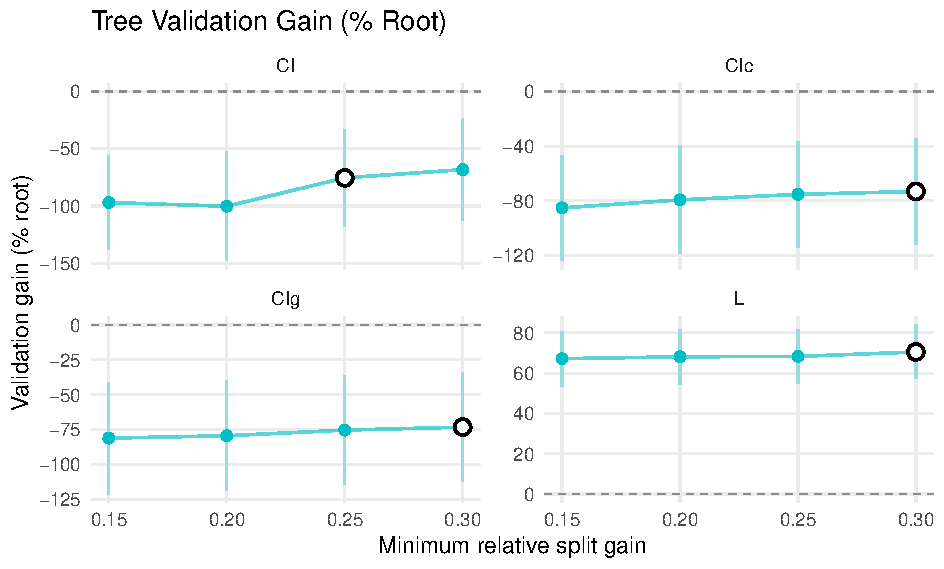
\includegraphics[keepaspectratio]{Decomposition_of_CI_Trees_MM_files/figure-pdf/fig-appendix-tree-validation-path-1.pdf}}

}

\caption{\label{fig-appendix-tree-validation-path}Tree validation gain
and complexity by minimum relative split gain.}

\end{figure}%

\subsubsection{Selected Concentration-Index
Tree}\label{selected-concentration-index-tree}

\begin{figure}[H]

\centering{

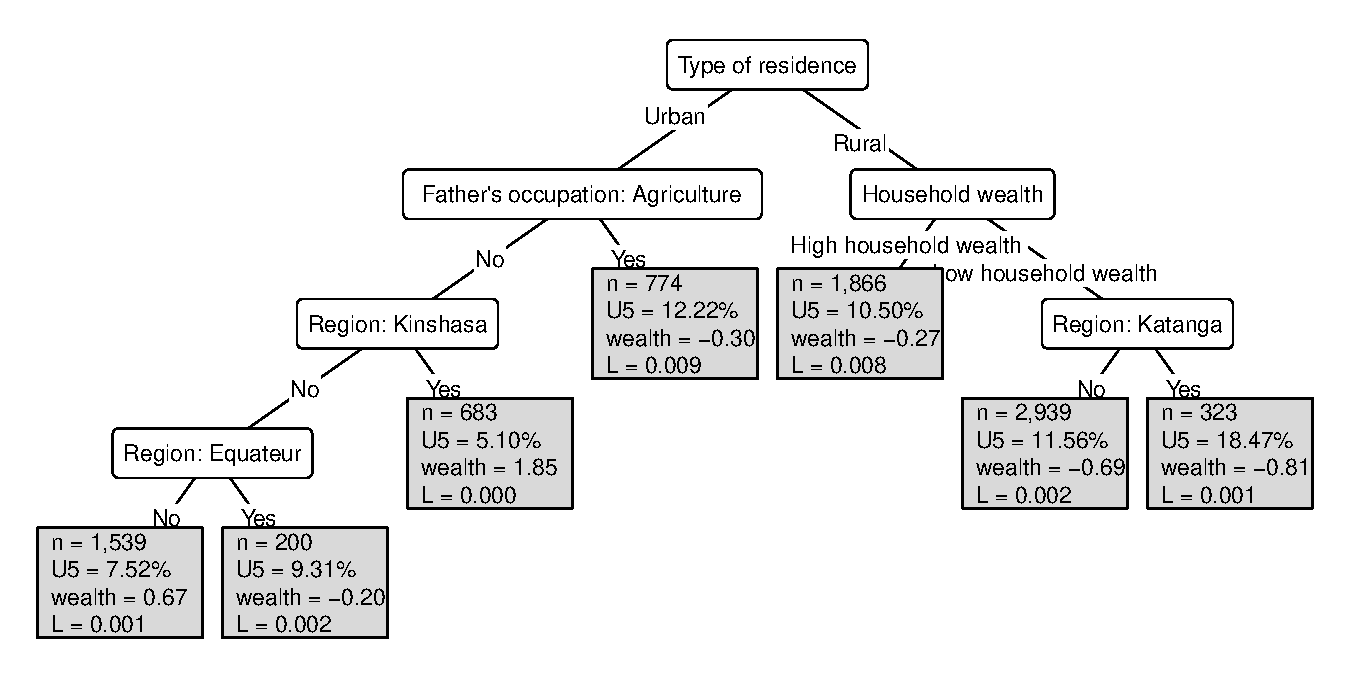
\includegraphics[width=1\linewidth,height=\textheight,keepaspectratio]{Decomposition_of_CI_Trees_MM_files/figure-pdf/fig-results-selected-ci-tree-1.pdf}

}

\caption{\label{fig-results-selected-ci-tree}Selected
concentration-index tree for under-five mortality in the DRC.}

\end{figure}%

\begin{figure}[H]

\centering{

\pandocbounded{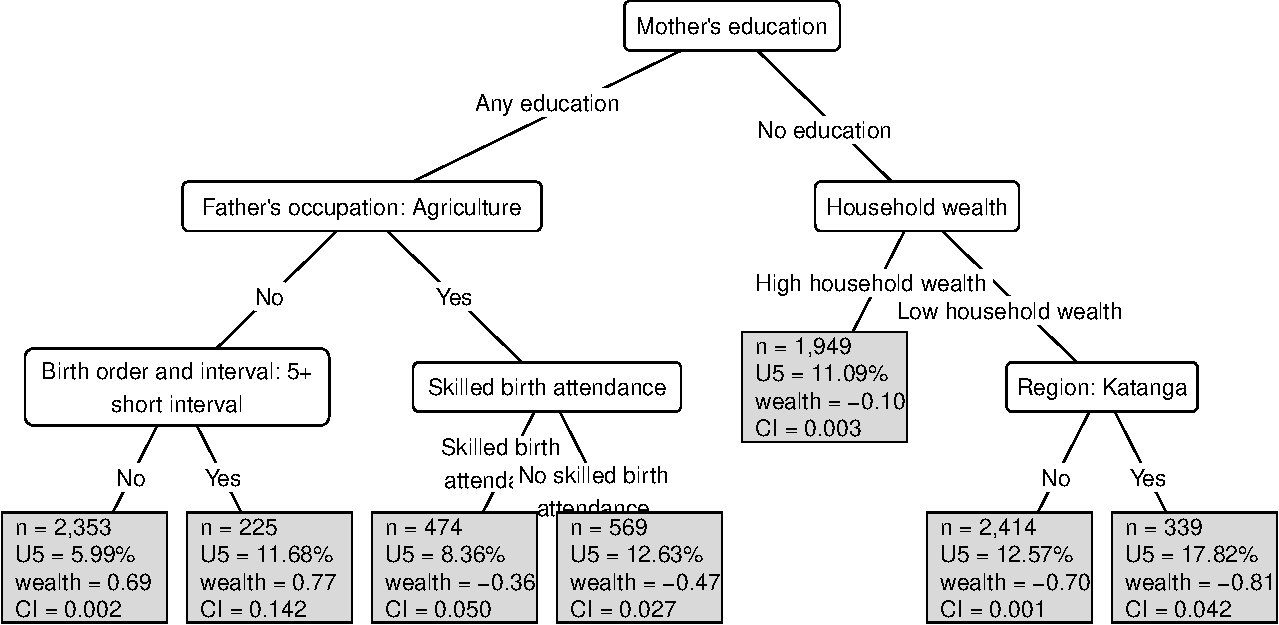
\includegraphics[keepaspectratio]{Decomposition_of_CI_Trees_MM_files/figure-pdf/fig-appendix-ci-tree-ci-1.pdf}}

}

\caption{\label{fig-appendix-ci-tree-ci}Concentration-index tree fitted
with the CI criterion.}

\end{figure}%

\subsubsection{Surrogate Tree
Comparison}\label{surrogate-tree-comparison}

\begin{figure}[H]

\centering{

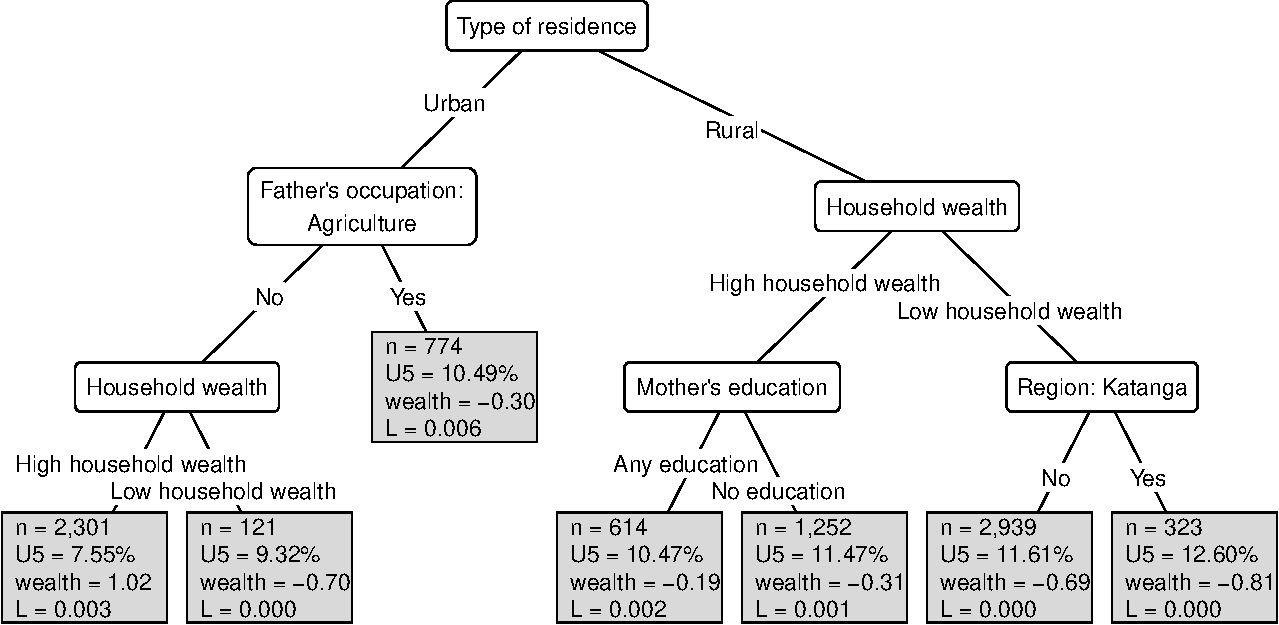
\includegraphics[width=1\linewidth,height=\textheight,keepaspectratio]{Decomposition_of_CI_Trees_MM_files/figure-pdf/fig-results-surrogate-tree-1.pdf}

}

\caption{\label{fig-results-surrogate-tree}Surrogate tree summarising
the selected concentration-index forest predictions.}

\end{figure}%

\begin{figure}[H]

\centering{

\pandocbounded{
\includegraphics[keepaspectratio]{Decomposition_of_CI_Trees_MM_files/figure-pdf/fig-results-selected-model-variable-importance-1.pdf}}

}

\caption{\label{fig-results-selected-model-variable-importance}Variable
importance for the selected concentration-index tree and forest.}

\end{figure}%

\subsection{Simulation Study}\label{simulation-study}

\subsubsection{Recovery of the Simulated Subgroup
Structure}\label{recovery-of-the-simulated-subgroup-structure}

The simulation study is used as a direct check on the tree-growing rule.
In the null simulation, wealth, the binary outcome, and the candidate
subgroup variables are generated independently. In the positive-control
simulation, the outcome is concentrated among poorer observations in a
planted subgroup defined by residence, maternal education, and province.
The null trees should therefore remain at the root node, while the
positive-control tree should recover a readable subgroup structure.

\begin{figure}[H]

\begin{minipage}[t]{0.50\linewidth}

\centering{

\pandocbounded{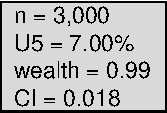
\includegraphics[keepaspectratio]{Decomposition_of_CI_Trees_MM_files/figure-pdf/fig-results-simulation-null-trees-1.pdf}}

}

\subcaption{\label{fig-results-simulation-null-trees-1}CI}

\end{minipage}%
%
\begin{minipage}[t]{0.50\linewidth}

\centering{

\pandocbounded{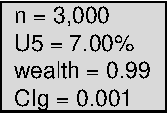
\includegraphics[keepaspectratio]{Decomposition_of_CI_Trees_MM_files/figure-pdf/fig-results-simulation-null-trees-2.pdf}}

}

\subcaption{\label{fig-results-simulation-null-trees-2}CIg}

\end{minipage}%
\newline
\begin{minipage}[t]{0.50\linewidth}

\centering{

\pandocbounded{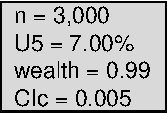
\includegraphics[keepaspectratio]{Decomposition_of_CI_Trees_MM_files/figure-pdf/fig-results-simulation-null-trees-3.pdf}}

}

\subcaption{\label{fig-results-simulation-null-trees-3}CIc}

\end{minipage}%
%
\begin{minipage}[t]{0.50\linewidth}

\centering{

\pandocbounded{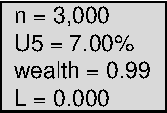
\includegraphics[keepaspectratio]{Decomposition_of_CI_Trees_MM_files/figure-pdf/fig-results-simulation-null-trees-4.pdf}}

}

\subcaption{\label{fig-results-simulation-null-trees-4}L}

\end{minipage}%

\caption{\label{fig-results-simulation-null-trees}Null simulation
concentration-index trees by criterion.}

\end{figure}%

\begin{figure}[H]

\centering{

\pandocbounded{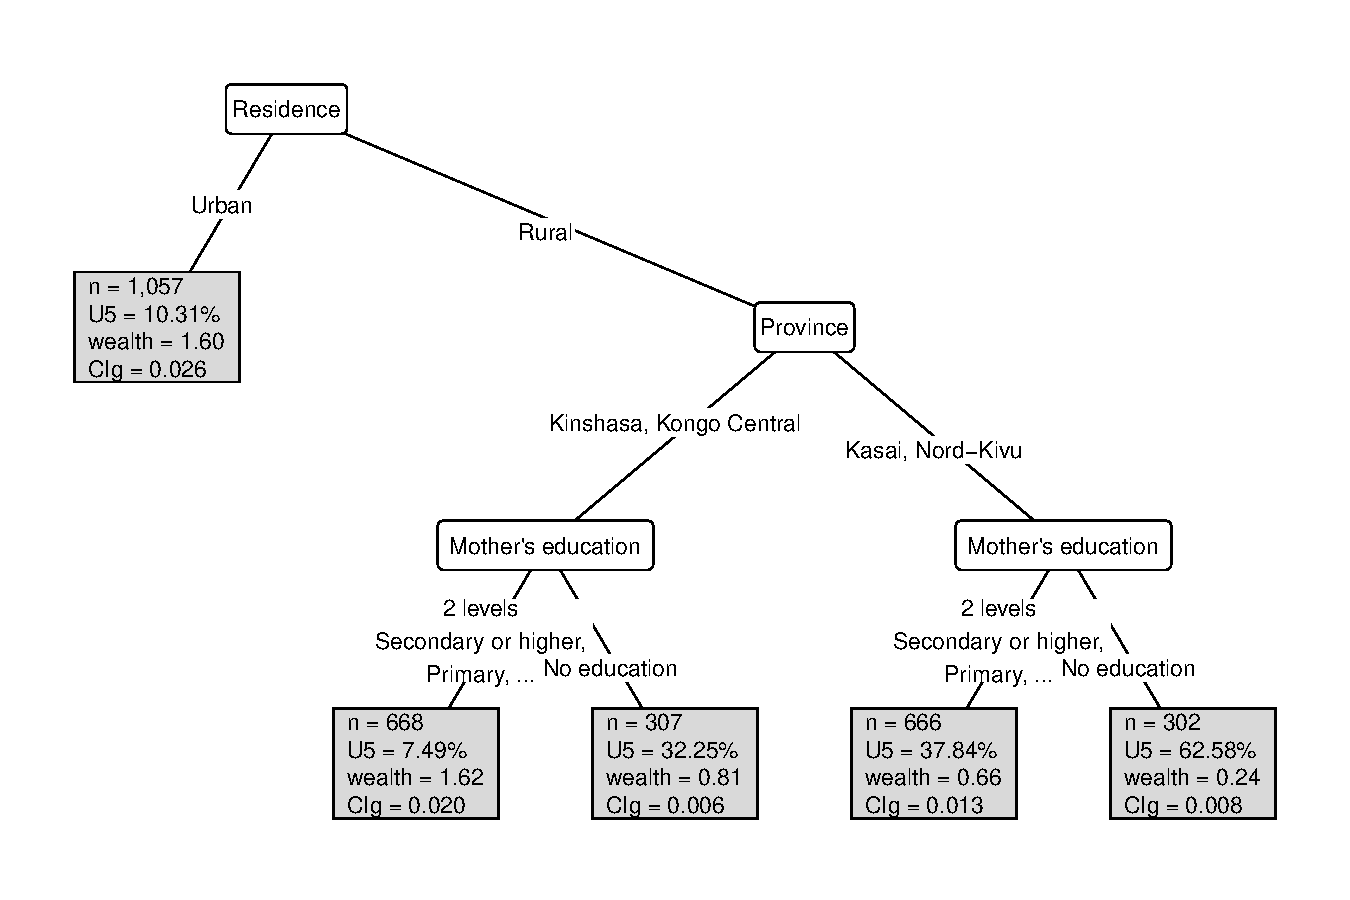
\includegraphics[keepaspectratio]{Decomposition_of_CI_Trees_MM_files/figure-pdf/fig-results-simulation-tree-1.pdf}}

}

\caption{\label{fig-results-simulation-tree}CIg concentration-index tree
recovered from simulated data with a known subgroup-generating
mechanism.}

\end{figure}%

\section{Appendix}\label{appendix}

\subsection{Results}\label{results-1}

\subsubsection{Appendix R1: Exploratory Data
Outputs}\label{appendix-r1-exploratory-data-outputs}

\begingroup\fontsize{11}{13}\selectfont

\begin{longtable}[t]{>{\raggedright\arraybackslash}p{4.5cm}>{\raggedleft\arraybackslash}p{3.1cm}>{\raggedleft\arraybackslash}p{3.1cm}>{\raggedleft\arraybackslash}p{3.1cm}}

\caption{\label{tbl-appendix-weighted-baseline}Weighted distribution of
analysis variables by under-five mortality status}

\tabularnewline

\\
\toprule
\multicolumn{1}{c}{\textbf{ }} & \multicolumn{2}{c}{\textbf{Under-five mortality}} & \multicolumn{1}{c}{\textbf{Overall}} \\
\cmidrule(l{3pt}r{3pt}){2-3} \cmidrule(l{3pt}r{3pt}){4-4}
\textbf{Variable} & \textbf{Alive at age 5} & \textbf{Died before age 5} & \textbf{Overall}\\
\midrule
 & (weighted N=7,464) & (weighted N=859) & (weighted N=8,323)\\
Household wealth &  &  & \\
High household wealth & 4,266.9 (57.2\%) & 418.6 (48.7\%) & 4,685.5 (56.3\%)\\
Low household wealth & 3,197.4 (42.8\%) & 440.2 (51.3\%) & 3,637.6 (43.7\%)\\
Skilled.birth.attendance &  &  & \\
\addlinespace
Skilled.birth.attendance.1 & 3,225.3 (43.2\%) & 295.1 (34.4\%) & 3,520.5 (42.3\%)\\
No.skilled.birth.attendance & 4,239 (56.8\%) & 563.6 (65.6\%) & 4,802.6 (57.7\%)\\
Sex of the child &  &  & \\
Female & 3,828.8 (51.3\%) & 390.4 (45.5\%) & 4,219.2 (50.7\%)\\
Male & 3,635.5 (48.7\%) & 468.4 (54.5\%) & 4,103.9 (49.3\%)\\
\addlinespace
Birth order and interval &  &  & \\
First birth & 1,396.8 (18.7\%) & 190.9 (22.2\%) & 1,587.7 (19.1\%)\\
2-4 short interval & 774.3 (10.4\%) & 110.1 (12.8\%) & 884.4 (10.6\%)\\
2-4 long interval & 2,603.8 (34.9\%) & 216.6 (25.2\%) & 2,820.3 (33.9\%)\\
5+ short interval & 696.6 (9.3\%) & 150.6 (17.5\%) & 847.2 (10.2\%)\\
\addlinespace
5+ long interval & 1,992.8 (26.7\%) & 190.7 (22.2\%) & 2,183.5 (26.2\%)\\
Mother's age at birth &  &  & \\
20 or more & 4,256.1 (57.0\%) & 472.6 (55.0\%) & 4,728.8 (56.8\%)\\
Less than 20 & 3,208.1 (43.0\%) & 386.2 (45.0\%) & 3,594.3 (43.2\%)\\
Type of residence &  &  & \\
\addlinespace
Urban & 2,932.1 (39.3\%) & 263.6 (30.7\%) & 3,195.7 (38.4\%)\\
Rural & 4,532.2 (60.7\%) & 595.2 (69.3\%) & 5,127.4 (61.6\%)\\
Mother's education &  &  & \\
Any education & 3,342.9 (44.8\%) & 278.8 (32.5\%) & 3,621.8 (43.5\%)\\
No education & 4,121.4 (55.2\%) & 579.9 (67.5\%) & 4,701.3 (56.5\%)\\
\addlinespace
Father's education &  &  & \\
Any education & 5,490 (73.6\%) & 589.1 (68.6\%) & 6,079.2 (73.0\%)\\
No education & 1,974.3 (26.4\%) & 269.7 (31.4\%) & 2,243.9 (27.0\%)\\
Mother's occupation &  &  & \\
Other & 1,610.2 (21.6\%) & 135.1 (15.7\%) & 1,745.4 (21.0\%)\\
\addlinespace
Household, unskilled, not working & 1,757.2 (23.5\%) & 172.1 (20.0\%) & 1,929.4 (23.2\%)\\
Agriculture & 4,096.8 (54.9\%) & 551.6 (64.2\%) & 4,648.4 (55.8\%)\\
Father's occupation &  &  & \\
Other & 2,810.3 (37.6\%) & 242.1 (28.2\%) & 3,052.4 (36.7\%)\\
Household, unskilled, not working & 961.3 (12.9\%) & 108.5 (12.6\%) & 1,069.8 (12.9\%)\\
\addlinespace
Agriculture & 3,692.7 (49.5\%) & 508.1 (59.2\%) & 4,200.9 (50.5\%)\\
\bottomrule

\end{longtable}

\endgroup{}

\begin{figure}[H]

\centering{

\pandocbounded{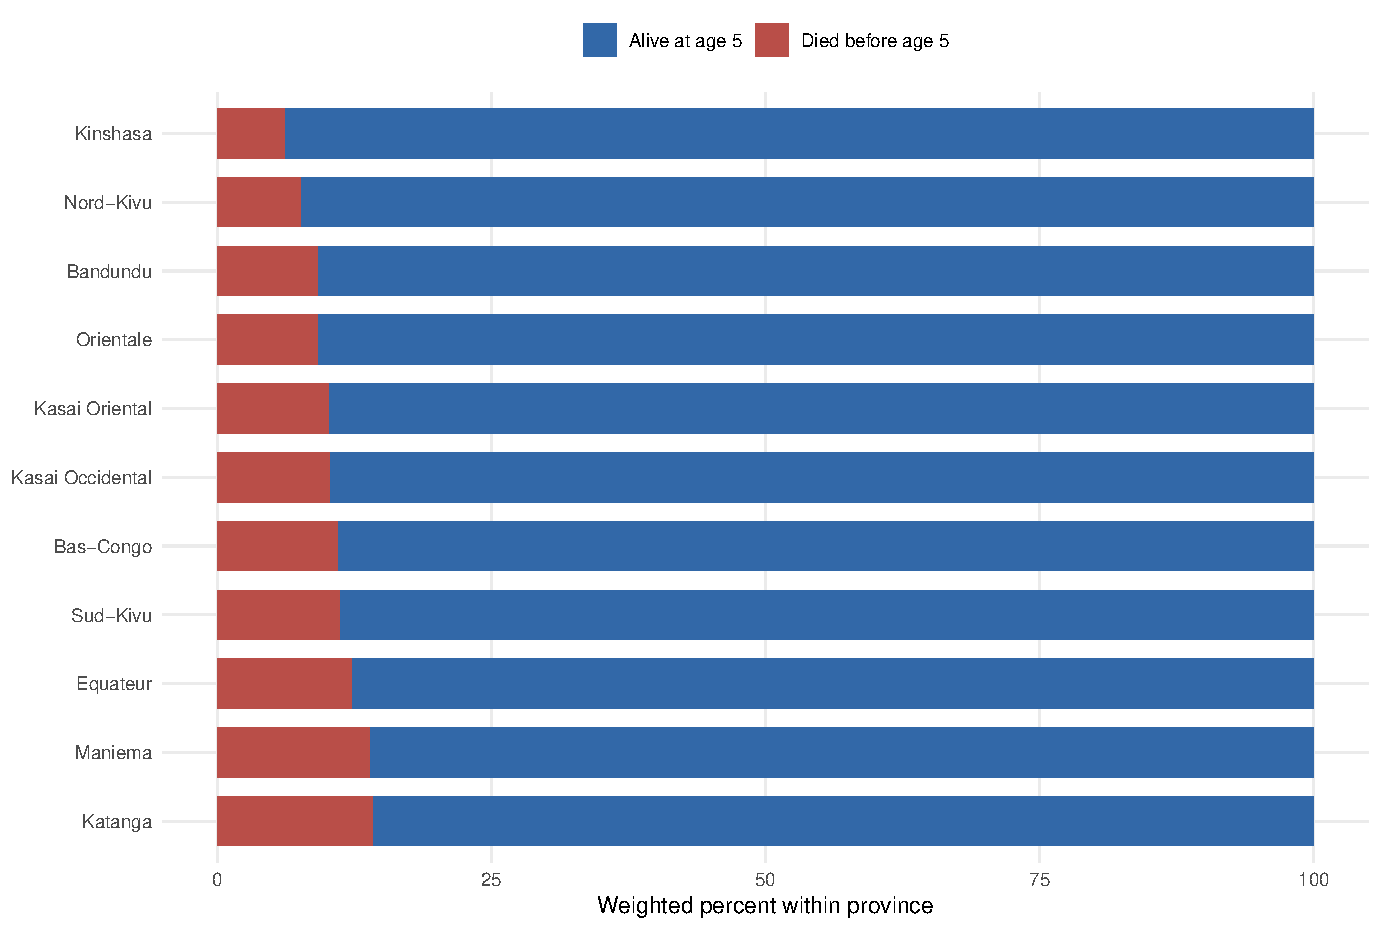
\includegraphics[keepaspectratio]{Decomposition_of_CI_Trees_MM_files/figure-pdf/fig-appendix-province-mortality-distribution-1.pdf}}

}

\caption{\label{fig-appendix-province-mortality-distribution}Weighted
province distribution by under-five mortality status.}

\end{figure}%

\subsubsection{Appendix R2: Regression and Predictive-Forest
Details}\label{appendix-r2-regression-and-predictive-forest-details}

\paragraph{Regression model summary}\label{regression-model-summary}

\begingroup\fontsize{11}{13}\selectfont

\begin{longtable}[t]{>{\raggedleft\arraybackslash}p{4.5cm}rrrrrr}

\caption{\label{tbl-appendix-regression-model-summary}Survey-weighted
regression model summary}

\tabularnewline

\\
\toprule
\textbf{Term} & \textbf{Estimate} & \textbf{Std. error} & \textbf{Statistic} & \textbf{p-value} & \textbf{Conf. low} & \textbf{Conf. high}\\
\midrule
Intercept & -2.908 & 0.275 & -10.563 & <0.001 & -3.448 & -2.369\\
Household wealth & 0.068 & 0.125 & 0.544 & 0.5865 & -0.177 & 0.314\\
Skilled birth attendance & 0.198 & 0.111 & 1.783 & 0.0746 & -0.020 & 0.416\\
Sex of the child & 0.242 & 0.105 & 2.294 & 0.0218 & 0.035 & 0.449\\
Birth order and interval: 2-4 short interval & -0.004 & 0.186 & -0.020 & 0.9838 & -0.367 & 0.360\\
\addlinespace
Birth order and interval: 2-4 long interval & -0.509 & 0.169 & -3.013 & 0.0026 & -0.840 & -0.178\\
Birth order and interval: 5+ short interval & 0.420 & 0.210 & 1.995 & 0.0461 & 0.007 & 0.832\\
Birth order and interval: 5+ long interval & -0.396 & 0.211 & -1.882 & 0.0599 & -0.809 & 0.017\\
Mother's age at birth & 0.033 & 0.143 & 0.229 & 0.8186 & -0.247 & 0.312\\
Type of residence & 0.090 & 0.154 & 0.584 & 0.5591 & -0.212 & 0.392\\
\addlinespace
Mother's education & 0.336 & 0.132 & 2.555 & 0.0106 & 0.078 & 0.594\\
Father's education & -0.036 & 0.128 & -0.280 & 0.7798 & -0.286 & 0.214\\
Mother's occupation: Household, unskilled, not working & -0.018 & 0.155 & -0.114 & 0.9093 & -0.322 & 0.287\\
Mother's occupation: Agriculture & 0.140 & 0.163 & 0.861 & 0.3895 & -0.180 & 0.460\\
Father's occupation: Household, unskilled, not working & 0.235 & 0.162 & 1.450 & 0.1472 & -0.083 & 0.554\\
\addlinespace
Father's occupation: Agriculture & 0.225 & 0.149 & 1.509 & 0.1314 & -0.067 & 0.517\\
Region: Bas-Congo & 0.258 & 0.243 & 1.062 & 0.2883 & -0.218 & 0.734\\
Region: Equateur & 0.250 & 0.238 & 1.051 & 0.2934 & -0.216 & 0.715\\
Region: Kasai Occidental & 0.105 & 0.228 & 0.460 & 0.6452 & -0.342 & 0.553\\
Region: Kasai Oriental & 0.153 & 0.240 & 0.635 & 0.5251 & -0.318 & 0.624\\
\addlinespace
Region: Katanga & 0.515 & 0.228 & 2.258 & 0.0240 & 0.068 & 0.962\\
Region: Kinshasa & 0.081 & 0.262 & 0.310 & 0.7564 & -0.433 & 0.596\\
Region: Maniema & 0.489 & 0.224 & 2.178 & 0.0294 & 0.049 & 0.929\\
Region: Nord-Kivu & -0.252 & 0.294 & -0.857 & 0.3915 & -0.827 & 0.324\\
Region: Orientale & -0.084 & 0.265 & -0.316 & 0.7522 & -0.603 & 0.435\\
\addlinespace
Region: Sud-Kivu & 0.300 & 0.270 & 1.111 & 0.2667 & -0.229 & 0.829\\
\bottomrule

\end{longtable}

\endgroup{}

\paragraph{Predictive ranger tuning
results}\label{predictive-ranger-tuning-results}

\begingroup\fontsize{11}{13}\selectfont

\begin{longtable}[t]{rrrrr}

\caption{\label{tbl-appendix-ranger-sampling-summary}Weighted class
distribution before and after ranger undersampling}

\tabularnewline

\\
\toprule
\textbf{Sample} & \textbf{Outcome} & \textbf{Rows} & \textbf{Weighted N} & \textbf{Weighted percent}\\
\midrule
Before undersampling & Alive at age 5 & 7424 & 7464.30 & 89.68\\
Before undersampling & Died before age 5 & 872 & 858.80 & 10.32\\
After undersampling & Alive at age 5 & 1274 & 1289.74 & 60.03\\
After undersampling & Died before age 5 & 872 & 858.80 & 39.97\\
\bottomrule

\end{longtable}

\endgroup{}

\begingroup\fontsize{11}{13}\selectfont

\begin{longtable}[t]{>{\raggedleft\arraybackslash}p{2.4cm}rrrrrr}

\caption{\label{tbl-appendix-ranger-cross-validation}Cross-validation
results for the predictive ranger model}

\tabularnewline

\\
\toprule
\textbf{Metric} & \textbf{mtry} & \textbf{min\_n} & \textbf{Mean} & \textbf{Std. error} & \textbf{Folds} & \textbf{Rank}\\
\midrule
accuracy & 19 & 1100 & 0.6123 & 0.0037 & 10 & 1\\
accuracy & 29 & 1100 & 0.6123 & 0.0042 & 10 & 2\\
accuracy & 10 & 200 & 0.6090 & 0.0093 & 10 & 3\\
accuracy & 29 & 200 & 0.6090 & 0.0106 & 10 & 4\\
accuracy & 10 & 1100 & 0.6081 & 0.0024 & 10 & 5\\
\addlinespace
accuracy & 19 & 200 & 0.6034 & 0.0094 & 10 & 6\\
accuracy & 1 & 200 & 0.5983 & 0.0014 & 10 & 7\\
accuracy & 1 & 1100 & 0.5937 & 0.0003 & 10 & 8\\
accuracy & 1 & 2000 & 0.5937 & 0.0003 & 10 & 9\\
accuracy & 10 & 2000 & 0.5937 & 0.0003 & 10 & 10\\
\addlinespace
accuracy & 19 & 2000 & 0.5937 & 0.0003 & 10 & 11\\
accuracy & 29 & 2000 & 0.5937 & 0.0003 & 10 & 12\\
roc\_auc & 1 & 200 & 0.6173 & 0.0118 & 10 & 1\\
roc\_auc & 10 & 200 & 0.6157 & 0.0110 & 10 & 2\\
roc\_auc & 1 & 1100 & 0.6147 & 0.0107 & 10 & 3\\
\addlinespace
roc\_auc & 29 & 200 & 0.6126 & 0.0103 & 10 & 4\\
roc\_auc & 19 & 200 & 0.6119 & 0.0103 & 10 & 5\\
roc\_auc & 10 & 1100 & 0.6069 & 0.0105 & 10 & 6\\
roc\_auc & 29 & 1100 & 0.6053 & 0.0108 & 10 & 7\\
roc\_auc & 19 & 1100 & 0.6047 & 0.0108 & 10 & 8\\
\addlinespace
roc\_auc & 1 & 2000 & 0.5000 & 0.0000 & 10 & 9\\
roc\_auc & 10 & 2000 & 0.5000 & 0.0000 & 10 & 10\\
roc\_auc & 19 & 2000 & 0.5000 & 0.0000 & 10 & 11\\
roc\_auc & 29 & 2000 & 0.5000 & 0.0000 & 10 & 12\\
sensitivity & 29 & 200 & 0.3072 & 0.0162 & 10 & 1\\
\addlinespace
sensitivity & 19 & 200 & 0.2854 & 0.0168 & 10 & 2\\
sensitivity & 10 & 200 & 0.2763 & 0.0159 & 10 & 3\\
sensitivity & 29 & 1100 & 0.1100 & 0.0105 & 10 & 4\\
sensitivity & 19 & 1100 & 0.0962 & 0.0134 & 10 & 5\\
sensitivity & 10 & 1100 & 0.0608 & 0.0086 & 10 & 6\\
\addlinespace
sensitivity & 1 & 200 & 0.0126 & 0.0036 & 10 & 7\\
sensitivity & 1 & 1100 & 0.0000 & 0.0000 & 10 & 8\\
sensitivity & 1 & 2000 & 0.0000 & 0.0000 & 10 & 9\\
sensitivity & 10 & 2000 & 0.0000 & 0.0000 & 10 & 10\\
sensitivity & 19 & 2000 & 0.0000 & 0.0000 & 10 & 11\\
\addlinespace
sensitivity & 29 & 2000 & 0.0000 & 0.0000 & 10 & 12\\
\bottomrule

\end{longtable}

\endgroup{}

\paragraph{Predictive ranger SHAP summary
plot}\label{predictive-ranger-shap-summary-plot}

\begin{figure}[H]

\centering{

\pandocbounded{
\includegraphics[keepaspectratio]{Decomposition_of_CI_Trees_MM_files/figure-pdf/fig-appendix-shap-summary-1.pdf}}

}

\caption{\label{fig-appendix-shap-summary}SHAP summary plot for the
predictive ranger model.}

\end{figure}%

\subsubsection{Appendix R3: Concentration-Index Tree
Details}\label{appendix-r3-concentration-index-tree-details}

\paragraph{Tree tuning and selection
details}\label{tree-tuning-and-selection-details}

\begingroup\fontsize{11}{13}\selectfont

\begin{longtable}[t]{rrrrrrr}

\caption{\label{tbl-appendix-tree-best-controls}Best tree
hyperparameters selected by validation gain within each impurity
criterion}

\tabularnewline

\\
\toprule
\textbf{type} & \textbf{minsplit} & \textbf{minbucket} & \textbf{minprob} & \textbf{maxdepth} & \textbf{min\_gain} & \textbf{min\_relative\_gain}\\
\midrule
CI & 500 & 100 & 0.01 & 10 & 1e-04 & 0.25\\
CIg & 500 & 100 & 0.01 & 10 & 1e-04 & 0.30\\
CIc & 500 & 100 & 0.01 & 10 & 1e-04 & 0.30\\
L & 500 & 100 & 0.01 & 10 & 1e-04 & 0.30\\
\bottomrule

\end{longtable}

\endgroup{}

\paragraph{Tree fit and selection
summaries}\label{tree-fit-and-selection-summaries}

\begingroup\fontsize{11}{13}\selectfont

\begin{longtable}[t]{rrrr}

\caption{\label{tbl-appendix-tree-selected-setting-summary}Tree summary
for the selected settings}

\tabularnewline

\\
\toprule
\textbf{criterion} & \textbf{metric} & \textbf{estimate} & \textbf{std\_error}\\
\midrule
CI & Root impurity & 0.1191 & NA\\
CI & Training gain & 0.1013 & 0.0017\\
CI & Training gain (\% root) & 87.9025 & 1.5310\\
CI & Validation gain & -0.0235 & 0.0220\\
CI & Validation gain (\% root) & -75.4763 & 42.7213\\
\addlinespace
CIc & Root impurity & 0.0483 & NA\\
CIc & Training gain & 0.0417 & 0.0008\\
CIc & Training gain (\% root) & 87.5995 & 1.4760\\
CIc & Validation gain & -0.0107 & 0.0134\\
CIc & Validation gain (\% root) & -73.1067 & 39.0032\\
\addlinespace
CIg & Root impurity & 0.0121 & NA\\
CIg & Training gain & 0.0104 & 0.0002\\
CIg & Training gain (\% root) & 87.5995 & 1.4760\\
CIg & Validation gain & -0.0027 & 0.0034\\
CIg & Validation gain (\% root) & -73.1067 & 39.0032\\
\addlinespace
L & Root impurity & 0.3128 & NA\\
L & Training gain & 0.1906 & 0.0061\\
L & Training gain (\% root) & 98.1536 & 0.2271\\
L & Validation gain & 0.2861 & 0.1077\\
L & Validation gain (\% root) & 70.5254 & 13.4254\\
\bottomrule

\end{longtable}

\endgroup{}

\paragraph{Tree selection metrics}\label{tree-selection-metrics}

\begingroup\fontsize{11}{13}\selectfont

\begin{longtable}[t]{>{\raggedleft\arraybackslash}p{1.4cm}>{\raggedleft\arraybackslash}p{1.8cm}>{\raggedleft\arraybackslash}p{1.8cm}>{\raggedleft\arraybackslash}p{1.8cm}>{\raggedleft\arraybackslash}p{1.8cm}>{\raggedleft\arraybackslash}p{1.8cm}>{\raggedleft\arraybackslash}p{1.8cm}}

\caption{\label{tbl-appendix-tree-selection}Selection metrics for fitted
concentration-index trees}

\tabularnewline

\\
\toprule
\textbf{Criterion} & \textbf{Root objective} & \textbf{Train gain} & \textbf{Train gain/root} & \textbf{Validation gain} & \textbf{Validation gain/root} & \textbf{Terminal nodes}\\
\midrule
CI & 0.1191 & 0.1013 & 0.8790 & -0.0235 & -0.7548 & 7.5\\
CIc & 0.0483 & 0.0417 & 0.8760 & -0.0107 & -0.7311 & 7.3\\
CIg & 0.0121 & 0.0104 & 0.8760 & -0.0027 & -0.7311 & 7.3\\
L & 0.3128 & 0.1906 & 0.9815 & 0.2861 & 0.7053 & 6.8\\
\bottomrule

\end{longtable}

\endgroup{}

\begin{figure}[H]

\centering{

\pandocbounded{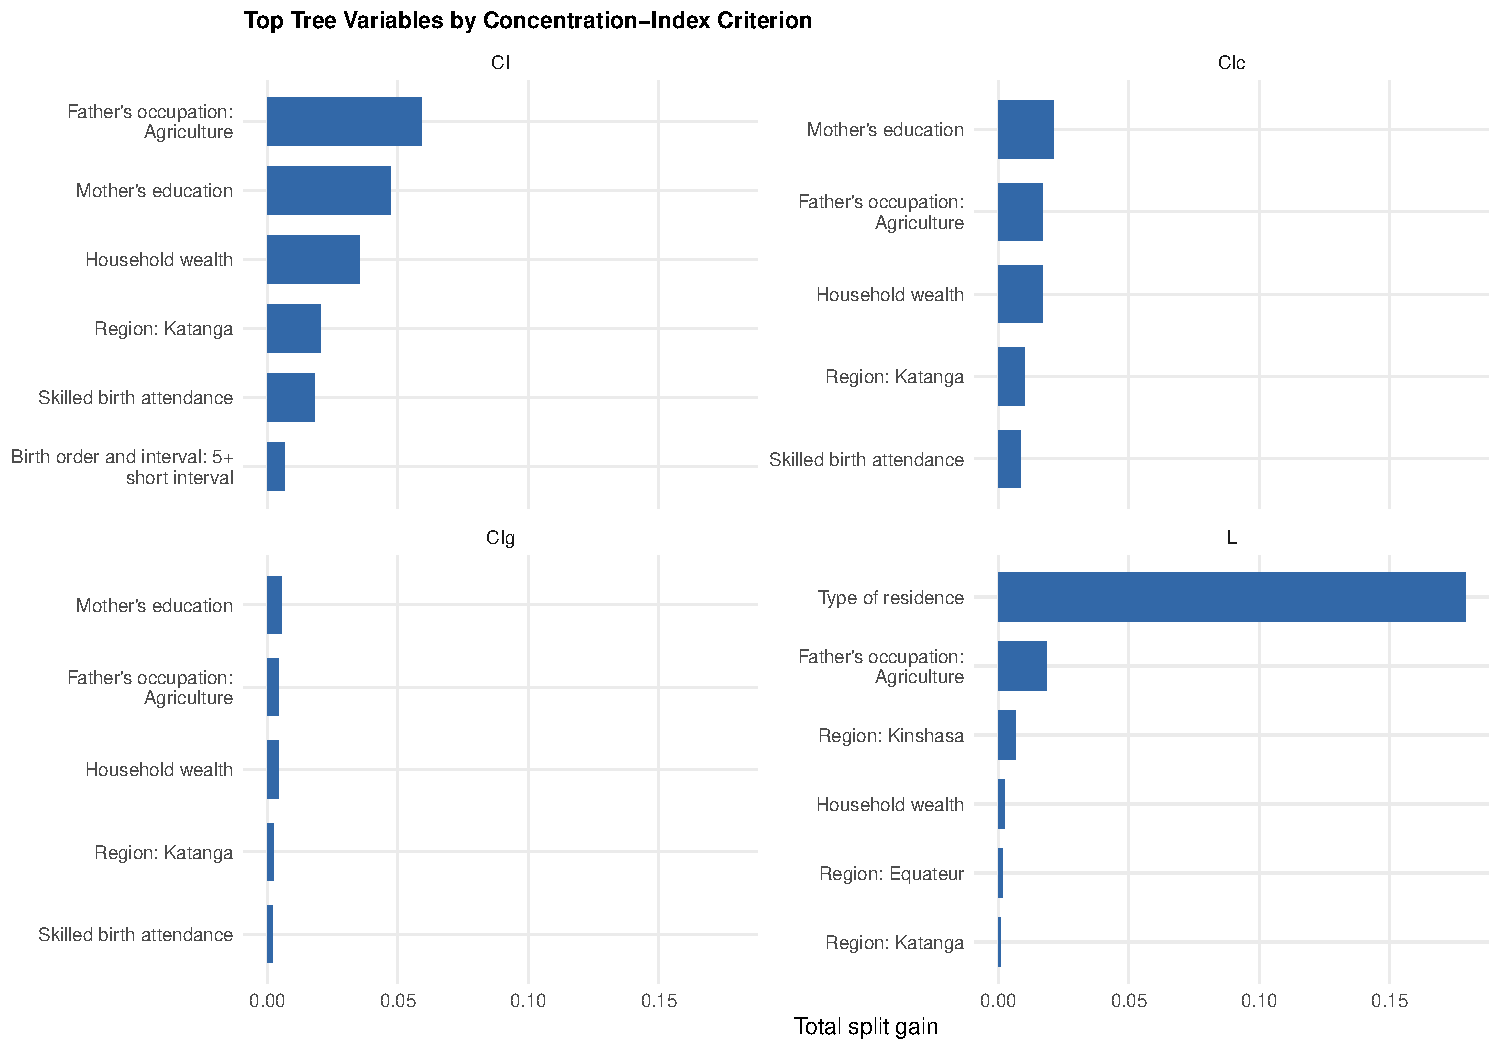
\includegraphics[keepaspectratio]{Decomposition_of_CI_Trees_MM_files/figure-pdf/fig-appendix-tree-variable-importance-1.pdf}}

}

\caption{\label{fig-appendix-tree-variable-importance}Top tree variables
by concentration-index criterion.}

\end{figure}%

\paragraph{Tree complexity plots}\label{tree-complexity-plots}

\begin{figure}[H]

\centering{

\pandocbounded{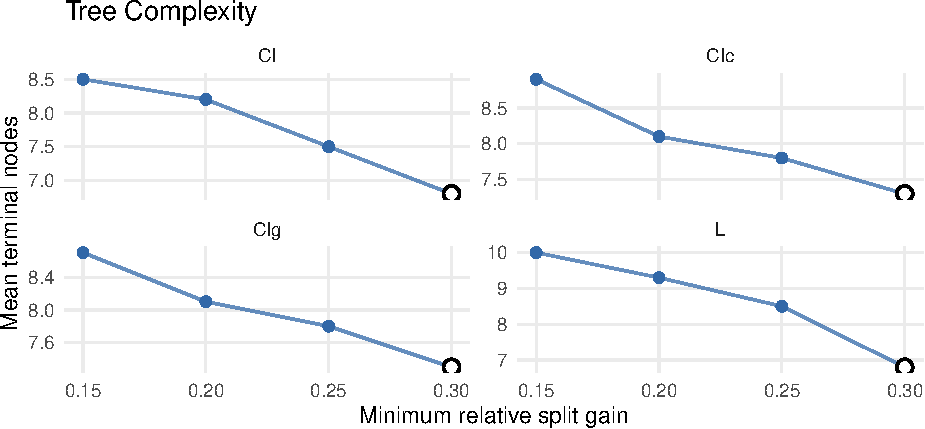
\includegraphics[keepaspectratio]{Decomposition_of_CI_Trees_MM_files/figure-pdf/fig-appendix-tree-complexity-path-1.pdf}}

}

\caption{\label{fig-appendix-tree-complexity-path}Tree complexity by
number of terminal nodes.}

\end{figure}%

\begin{figure}[H]

\centering{

\pandocbounded{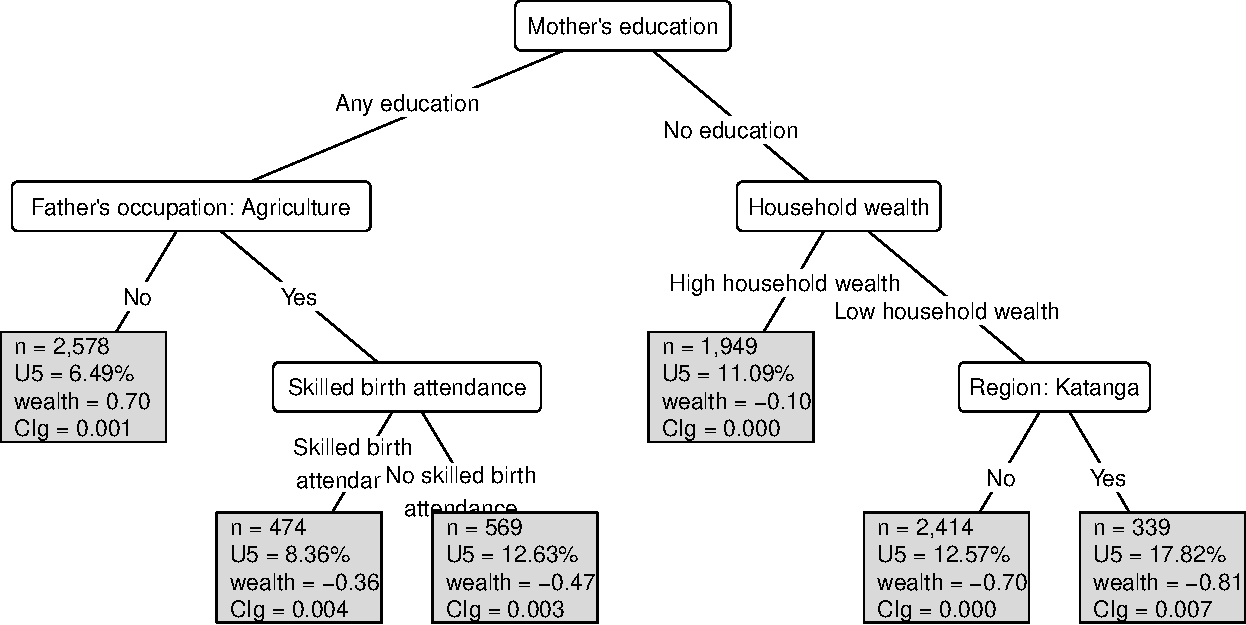
\includegraphics[keepaspectratio]{Decomposition_of_CI_Trees_MM_files/figure-pdf/fig-appendix-ci-tree-cig-1.pdf}}

}

\caption{\label{fig-appendix-ci-tree-cig}Concentration-index tree fitted
with the CIg criterion.}

\end{figure}%

\begin{figure}[H]

\centering{

\pandocbounded{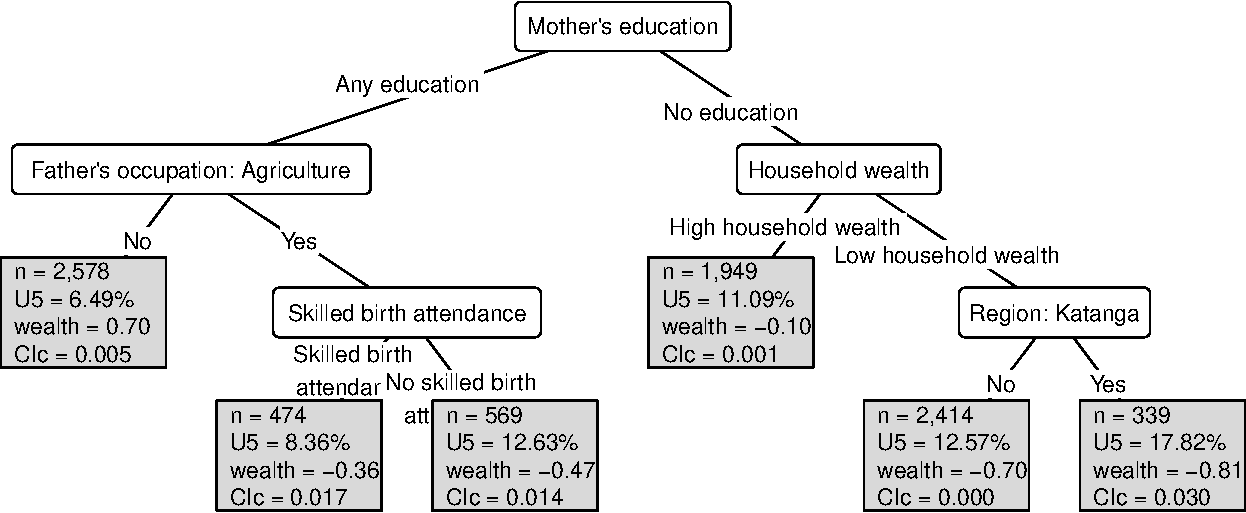
\includegraphics[keepaspectratio]{Decomposition_of_CI_Trees_MM_files/figure-pdf/fig-appendix-ci-tree-cic-1.pdf}}

}

\caption{\label{fig-appendix-ci-tree-cic}Concentration-index tree fitted
with the CIc criterion.}

\end{figure}%

\subsubsection{Appendix R4: Rpart Comparison Tree
Details}\label{appendix-r4-rpart-comparison-tree-details}

\begin{figure}[H]

\centering{

\pandocbounded{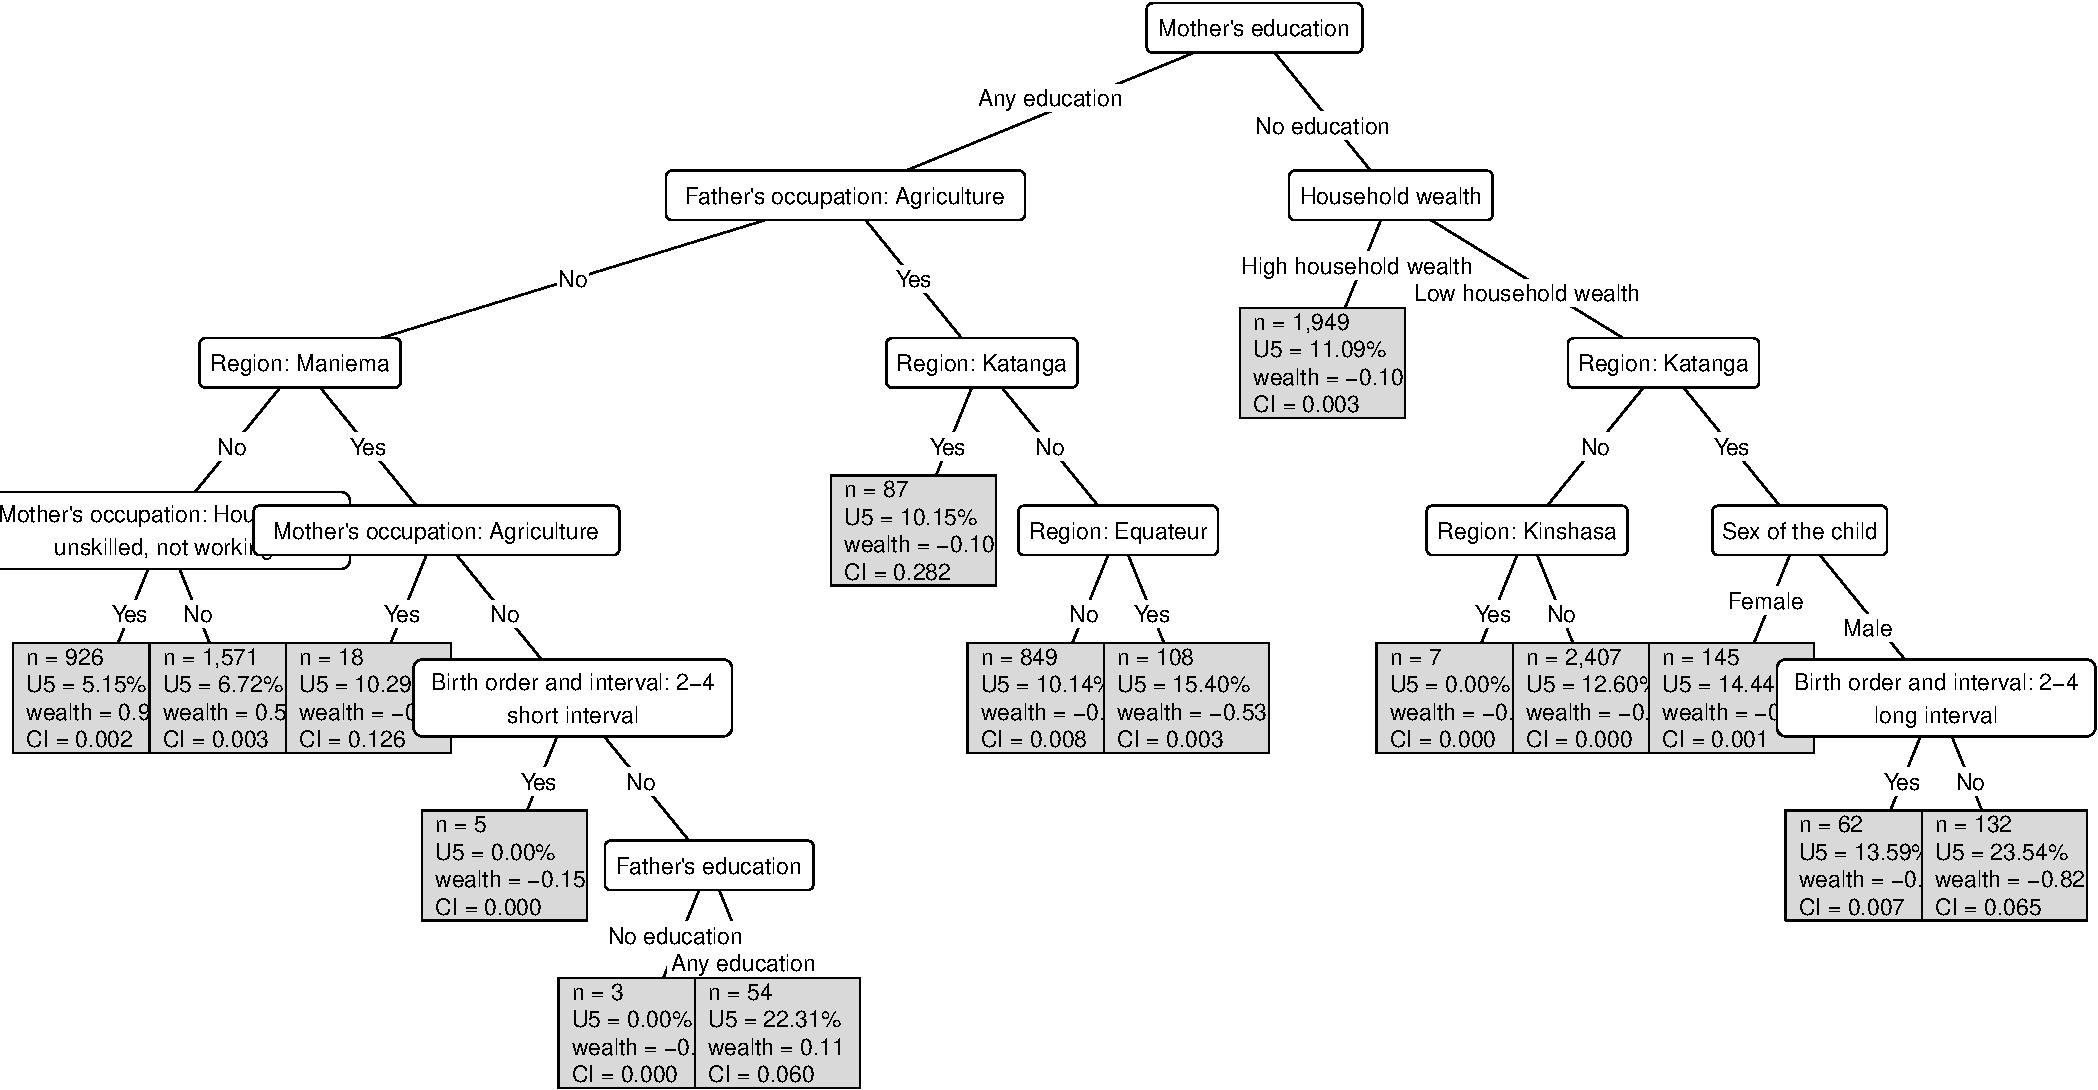
\includegraphics[keepaspectratio]{Decomposition_of_CI_Trees_MM_files/figure-pdf/fig-appendix-lecturer-rpart-simple-1.pdf}}

}

\caption{\label{fig-appendix-lecturer-rpart-simple}Lecturer rpart
comparison tree using absolute CI impurity.}

\end{figure}%

\begin{figure}[H]

\centering{

\pandocbounded{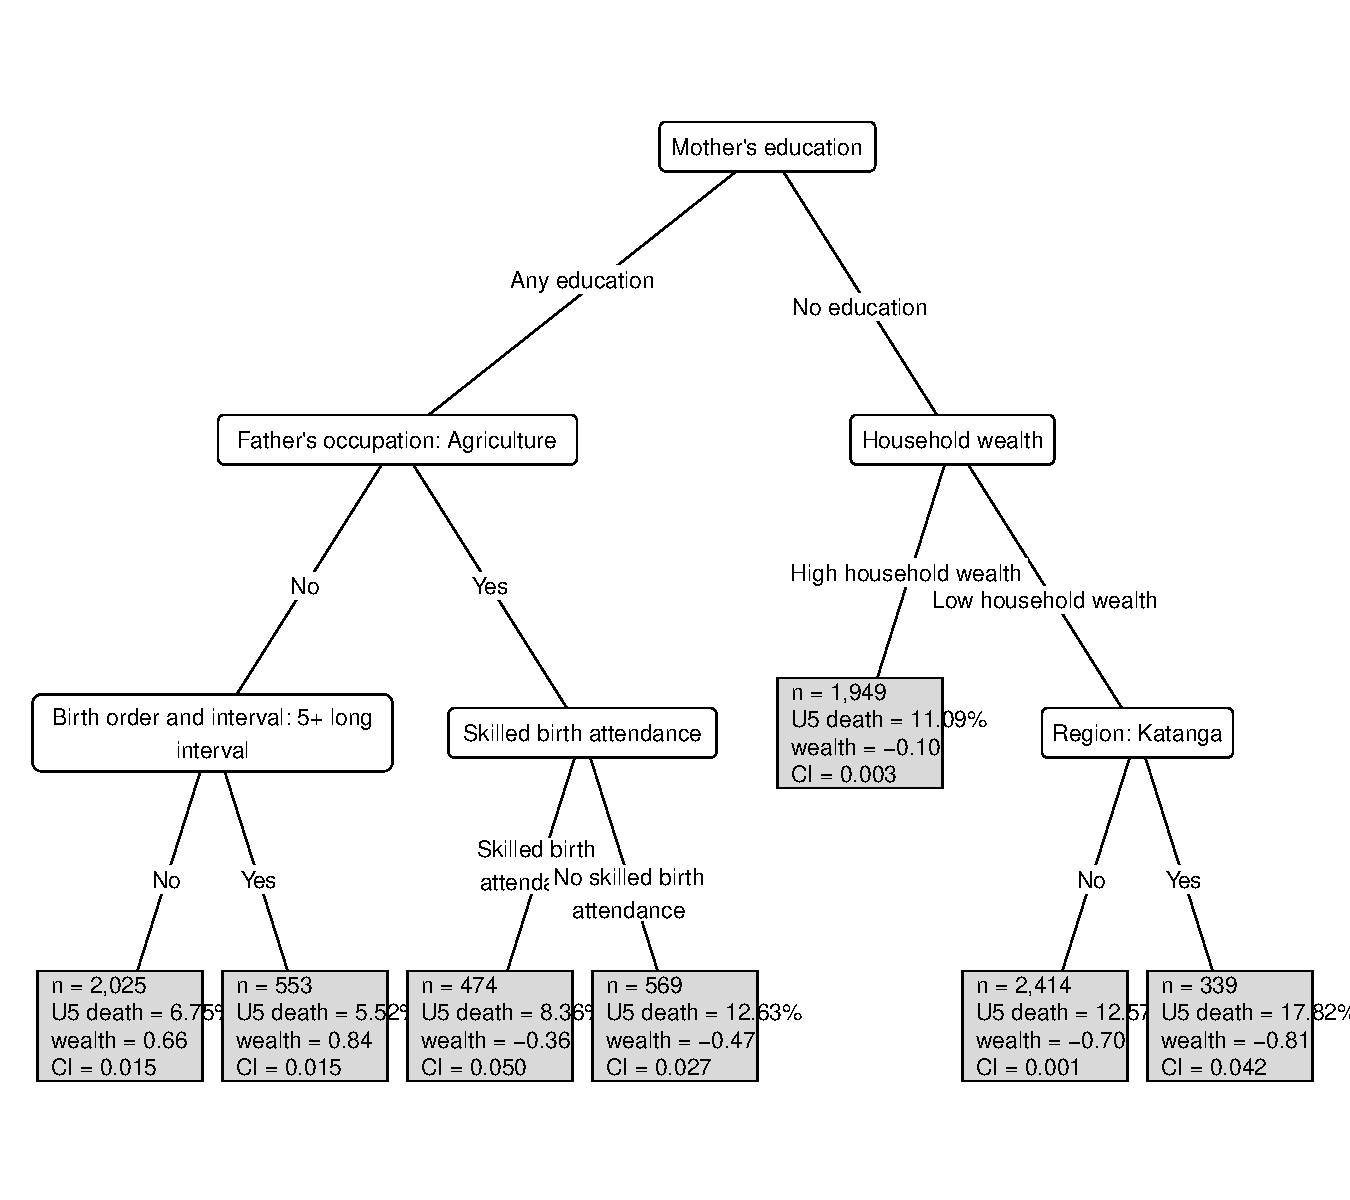
\includegraphics[keepaspectratio]{Decomposition_of_CI_Trees_MM_files/figure-pdf/fig-appendix-lecturer-rpart-robust-1.pdf}}

}

\caption{\label{fig-appendix-lecturer-rpart-robust}Lecturer rpart
comparison tree using robust absolute CI impurity.}

\end{figure}%

\subsubsection{Appendix 5: Concentration-Index Forest
Details}\label{appendix-5-concentration-index-forest-details}

\paragraph{Forest tuning and selection
details}\label{forest-tuning-and-selection-details}

\begingroup\fontsize{11}{13}\selectfont

\begin{longtable}[t]{rrrrrrrrr}

\caption{\label{tbl-appendix-forest-best-controls}Best forest
hyperparameters selected by validation gain within each impurity
criterion}

\tabularnewline

\\
\toprule
\textbf{type} & \textbf{ntree} & \textbf{mtry} & \textbf{minsplit} & \textbf{minbucket} & \textbf{minprob} & \textbf{maxdepth} & \textbf{min\_gain} & \textbf{min\_relative\_gain}\\
\midrule
CI & 50 & 10 & 500 & 100 & 0.01 & 15 & 0 & 0.35\\
CIc & 50 & 10 & 500 & 100 & 0.01 & 15 & 0 & 0.30\\
CIg & 50 & 10 & 500 & 100 & 0.01 & 15 & 0 & 0.25\\
L & 50 & 10 & 500 & 100 & 0.01 & 15 & 0 & 0.40\\
\bottomrule

\end{longtable}

\endgroup{}

\paragraph{Forest fit and selection
summaries}\label{forest-fit-and-selection-summaries}

\begingroup\fontsize{11}{13}\selectfont

\begin{longtable}[t]{rrrr}

\caption{\label{tbl-appendix-forest-selected-setting-summary}Forest
summary for the selected settings}

\tabularnewline

\\
\toprule
\textbf{criterion} & \textbf{metric} & \textbf{estimate} & \textbf{std\_error}\\
\midrule
CI & Root impurity & 0.1191 & NA\\
CI & Training gain & 0.0222 & 0.0027\\
CI & Training gain (\% root) & 19.4745 & 2.4825\\
CI & Validation gain & -0.0032 & 0.0077\\
CI & Validation gain (\% root) & -13.8147 & 8.1216\\
\addlinespace
CIc & Root impurity & 0.0483 & NA\\
CIc & Training gain & 0.0167 & 0.0007\\
CIc & Training gain (\% root) & 35.0907 & 1.5278\\
CIc & Validation gain & -0.0041 & 0.0052\\
CIc & Validation gain (\% root) & -37.0209 & 19.7261\\
\addlinespace
CIg & Root impurity & 0.0121 & NA\\
CIg & Training gain & 0.0047 & 0.0002\\
CIg & Training gain (\% root) & 39.8170 & 1.2803\\
CIg & Validation gain & -0.0010 & 0.0014\\
CIg & Validation gain (\% root) & -37.6958 & 20.8545\\
\addlinespace
L & Root impurity & 0.3128 & NA\\
L & Training gain & 0.1803 & 0.0059\\
L & Training gain (\% root) & 92.8313 & 0.4426\\
L & Validation gain & 0.2803 & 0.1025\\
L & Validation gain (\% root) & 71.8405 & 13.3582\\
\bottomrule

\end{longtable}

\endgroup{}

\paragraph{Forest selection metrics}\label{forest-selection-metrics}

\begingroup\fontsize{11}{13}\selectfont

\begin{longtable}[t]{>{\raggedleft\arraybackslash}p{1.4cm}>{\raggedleft\arraybackslash}p{1.8cm}>{\raggedleft\arraybackslash}p{1.8cm}>{\raggedleft\arraybackslash}p{1.8cm}>{\raggedleft\arraybackslash}p{1.8cm}>{\raggedleft\arraybackslash}p{1.8cm}>{\raggedleft\arraybackslash}p{1.8cm}}

\caption{\label{tbl-appendix-forest-selection}Selection metrics for
fitted concentration-index forests}

\tabularnewline

\\
\toprule
\textbf{Criterion} & \textbf{Root objective} & \textbf{Train gain} & \textbf{Train gain/root} & \textbf{Validation gain} & \textbf{Validation gain/root} & \textbf{Mean terminal nodes}\\
\midrule
CI & 0.1191 & 0.0222 & 0.1947 & -0.0032 & -0.1381 & 1.846\\
CIc & 0.0483 & 0.0167 & 0.3509 & -0.0041 & -0.3702 & 2.700\\
CIg & 0.0121 & 0.0047 & 0.3982 & -0.0010 & -0.3770 & 3.196\\
L & 0.3128 & 0.1803 & 0.9283 & 0.2803 & 0.7184 & 3.270\\
\bottomrule

\end{longtable}

\endgroup{}

\paragraph{Forest validation plots}\label{forest-validation-plots}

\begin{figure}[H]

\centering{

\pandocbounded{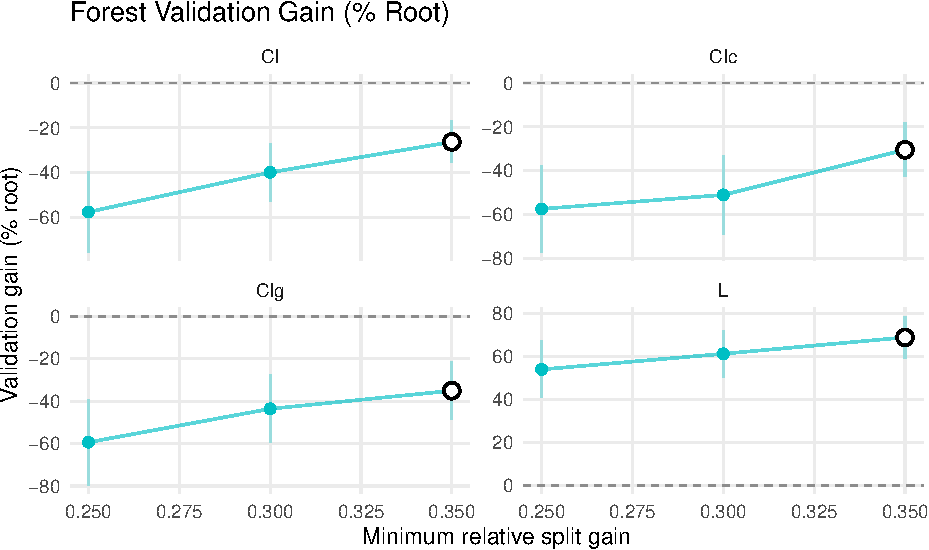
\includegraphics[keepaspectratio]{Decomposition_of_CI_Trees_MM_files/figure-pdf/fig-appendix-forest-validation-path-1.pdf}}

}

\caption{\label{fig-appendix-forest-validation-path}Forest validation
gain and complexity by minimum relative split gain.}

\end{figure}%

\paragraph{Forest complexity plots}\label{forest-complexity-plots}

\begin{figure}[H]

\centering{

\pandocbounded{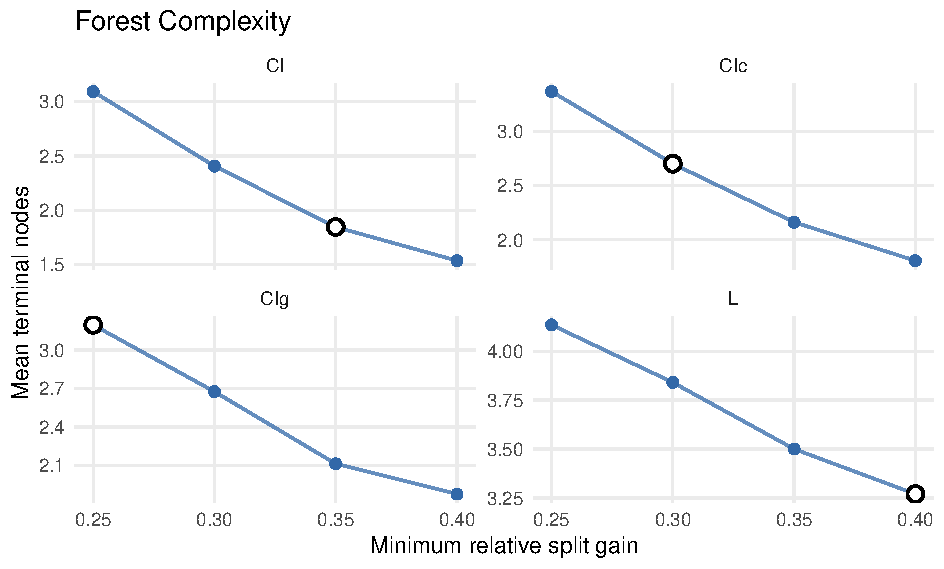
\includegraphics[keepaspectratio]{Decomposition_of_CI_Trees_MM_files/figure-pdf/fig-appendix-forest-complexity-path-1.pdf}}

}

\caption{\label{fig-appendix-forest-complexity-path}Forest complexity by
number of terminal nodes.}

\end{figure}%

\begin{figure}[H]

\centering{

\pandocbounded{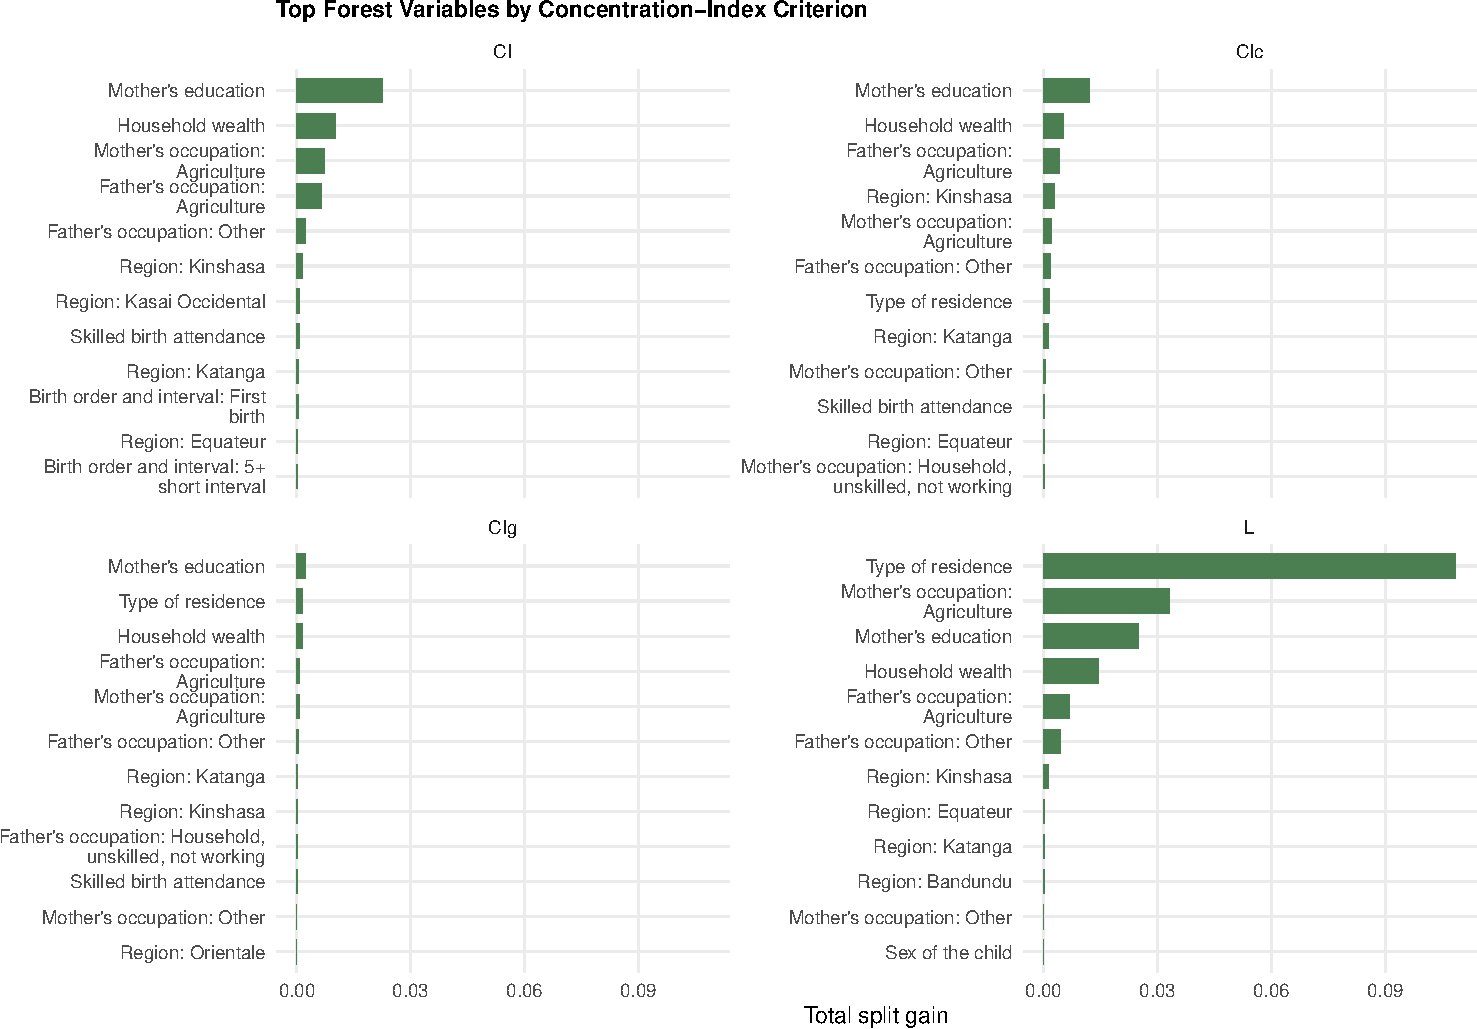
\includegraphics[keepaspectratio]{Decomposition_of_CI_Trees_MM_files/figure-pdf/fig-appendix-forest-variable-importance-1.pdf}}

}

\caption{\label{fig-appendix-forest-variable-importance}Top forest
variables by concentration-index criterion.}

\end{figure}%

\paragraph{Forest Surrogate Trees
plots}\label{forest-surrogate-trees-plots}

The selected forest surrogate appears in the results section. The
remaining criterion-specific forest surrogates are retained here for
comparison.

\begin{figure}[H]

\centering{

\pandocbounded{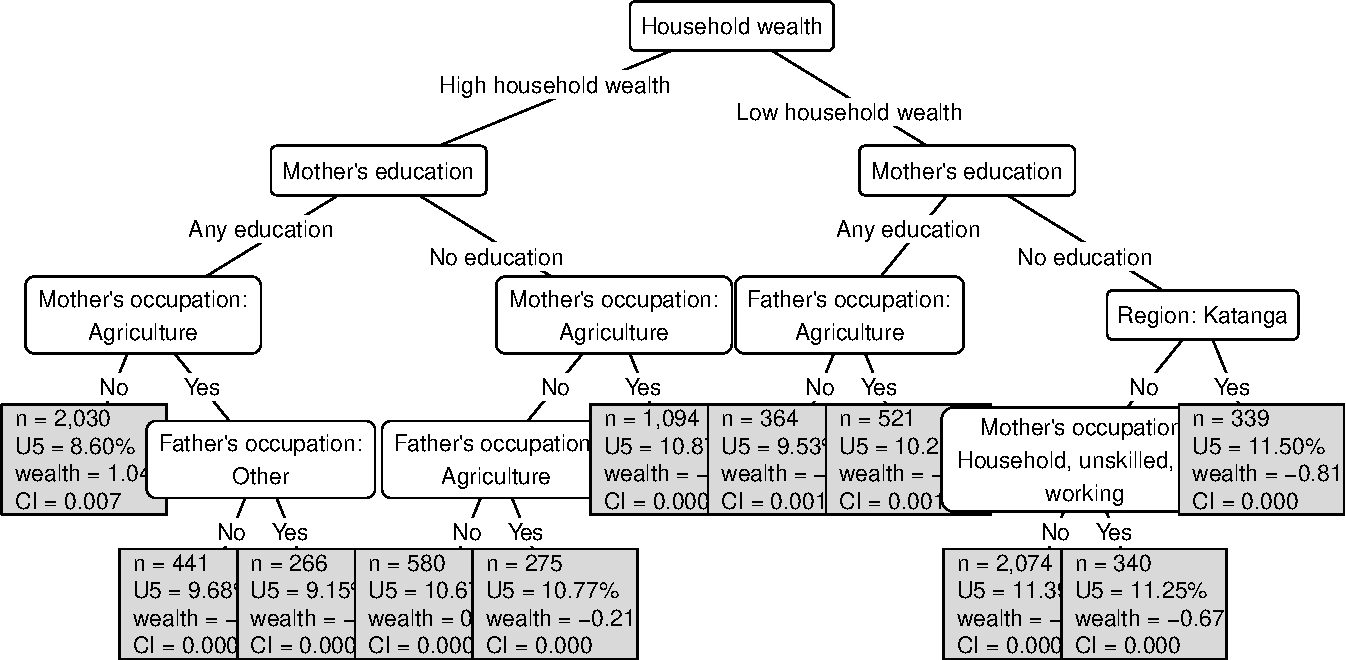
\includegraphics[keepaspectratio]{Decomposition_of_CI_Trees_MM_files/figure-pdf/fig-appendix-forest-surrogate-ci-1.pdf}}

}

\caption{\label{fig-appendix-forest-surrogate-ci}Surrogate tree for the
CI concentration-index forest.}

\end{figure}%

\begin{figure}[H]

\centering{

\pandocbounded{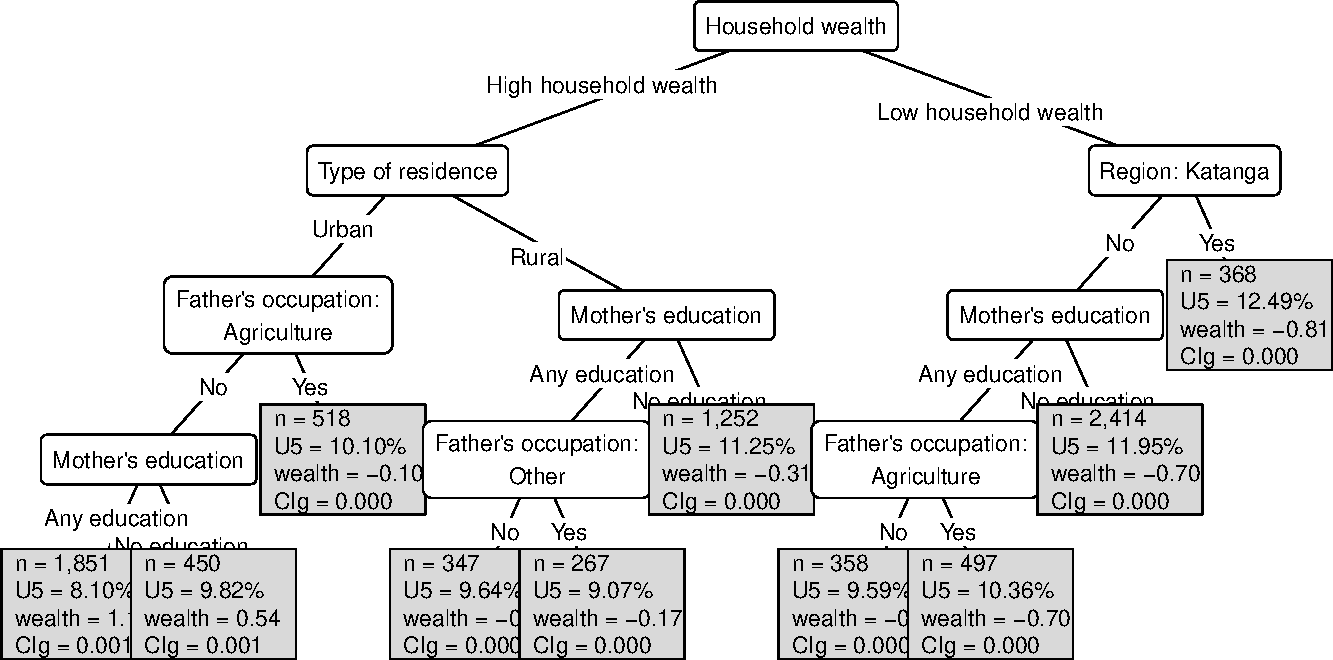
\includegraphics[keepaspectratio]{Decomposition_of_CI_Trees_MM_files/figure-pdf/fig-appendix-forest-surrogate-cig-1.pdf}}

}

\caption{\label{fig-appendix-forest-surrogate-cig}Surrogate tree for the
CIg concentration-index forest.}

\end{figure}%

\begin{figure}[H]

\centering{

\pandocbounded{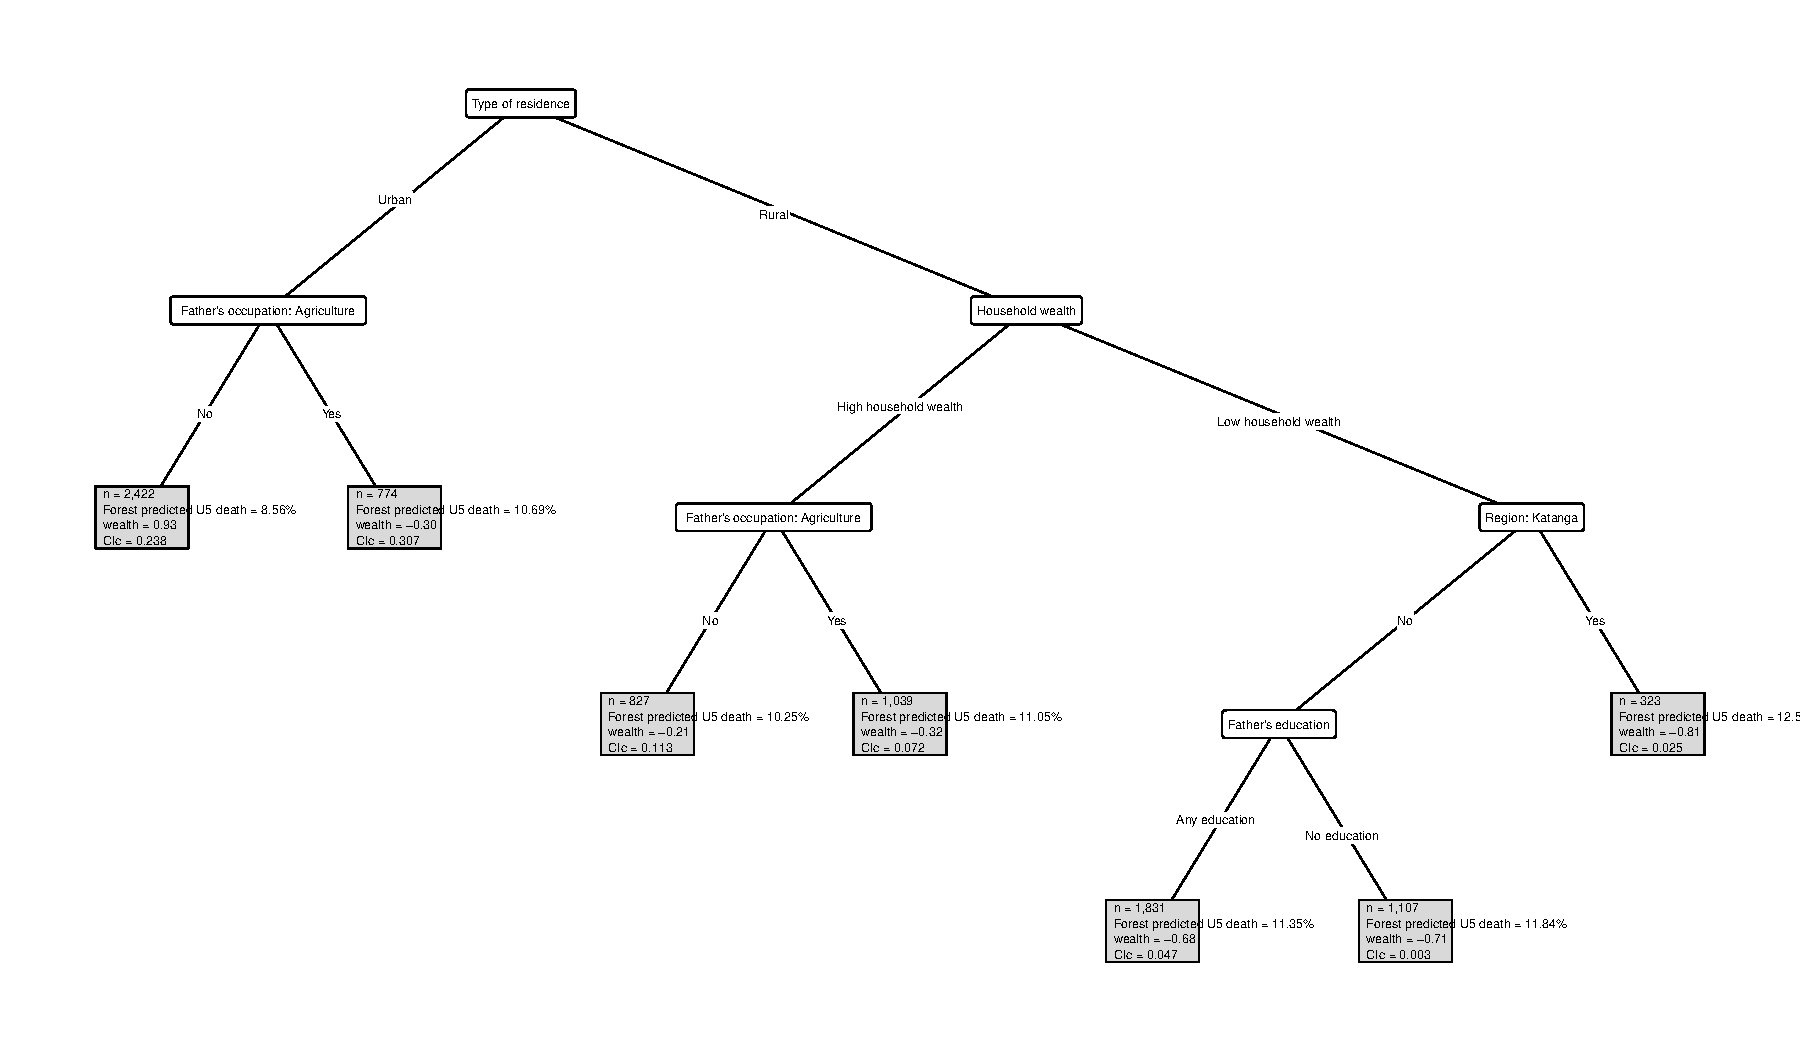
\includegraphics[keepaspectratio]{Decomposition_of_CI_Trees_MM_files/figure-pdf/fig-appendix-forest-surrogate-cic-1.pdf}}

}

\caption{\label{fig-appendix-forest-surrogate-cic}Surrogate tree for the
CIc concentration-index forest.}

\end{figure}%

\subsubsection{Appendix S: Simulation Sensitivity
Plots}\label{appendix-s-simulation-sensitivity-plots}

The CIg tree is shown in the main results section. The remaining
positive-control simulation trees are shown here to check whether the
recovered subgroup pattern is stable across concentration-index
criteria.

\begin{figure}[H]

\centering{

\pandocbounded{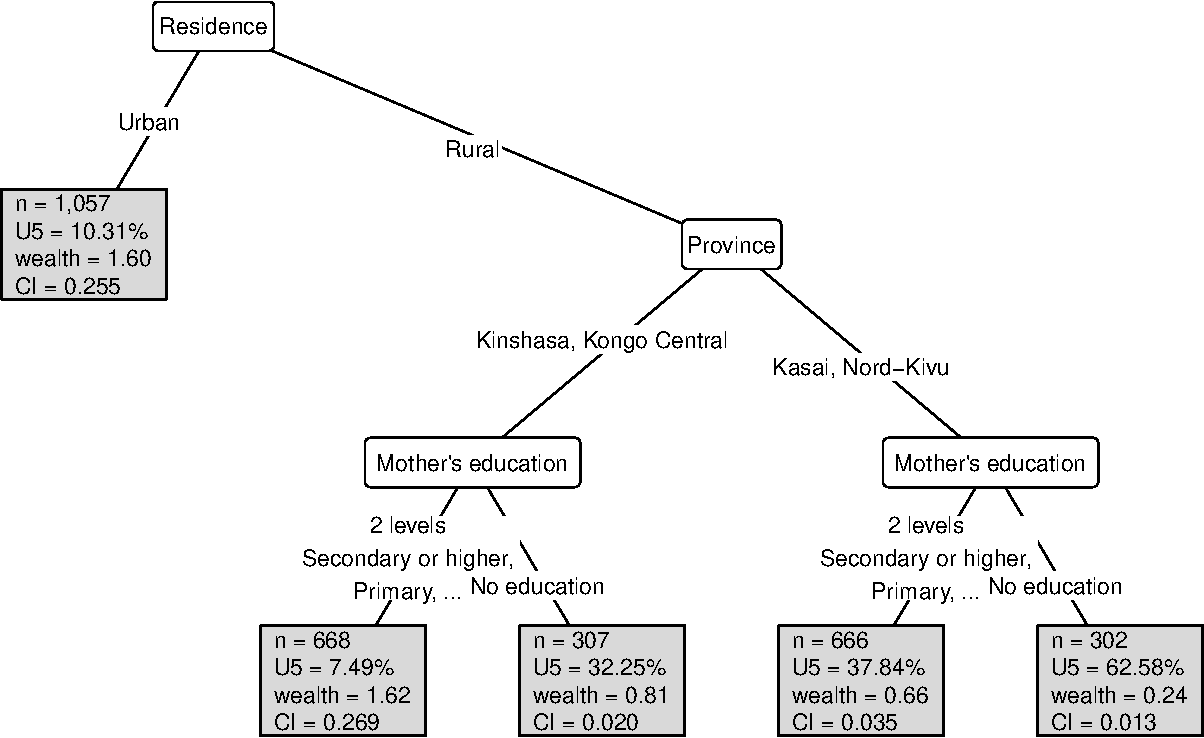
\includegraphics[keepaspectratio]{Decomposition_of_CI_Trees_MM_files/figure-pdf/fig-appendix-simulation-positive-control-ci-1.pdf}}

}

\caption{\label{fig-appendix-simulation-positive-control-ci}Positive-control
simulation tree fitted with the CI criterion.}

\end{figure}%

\begin{figure}[H]

\centering{

\pandocbounded{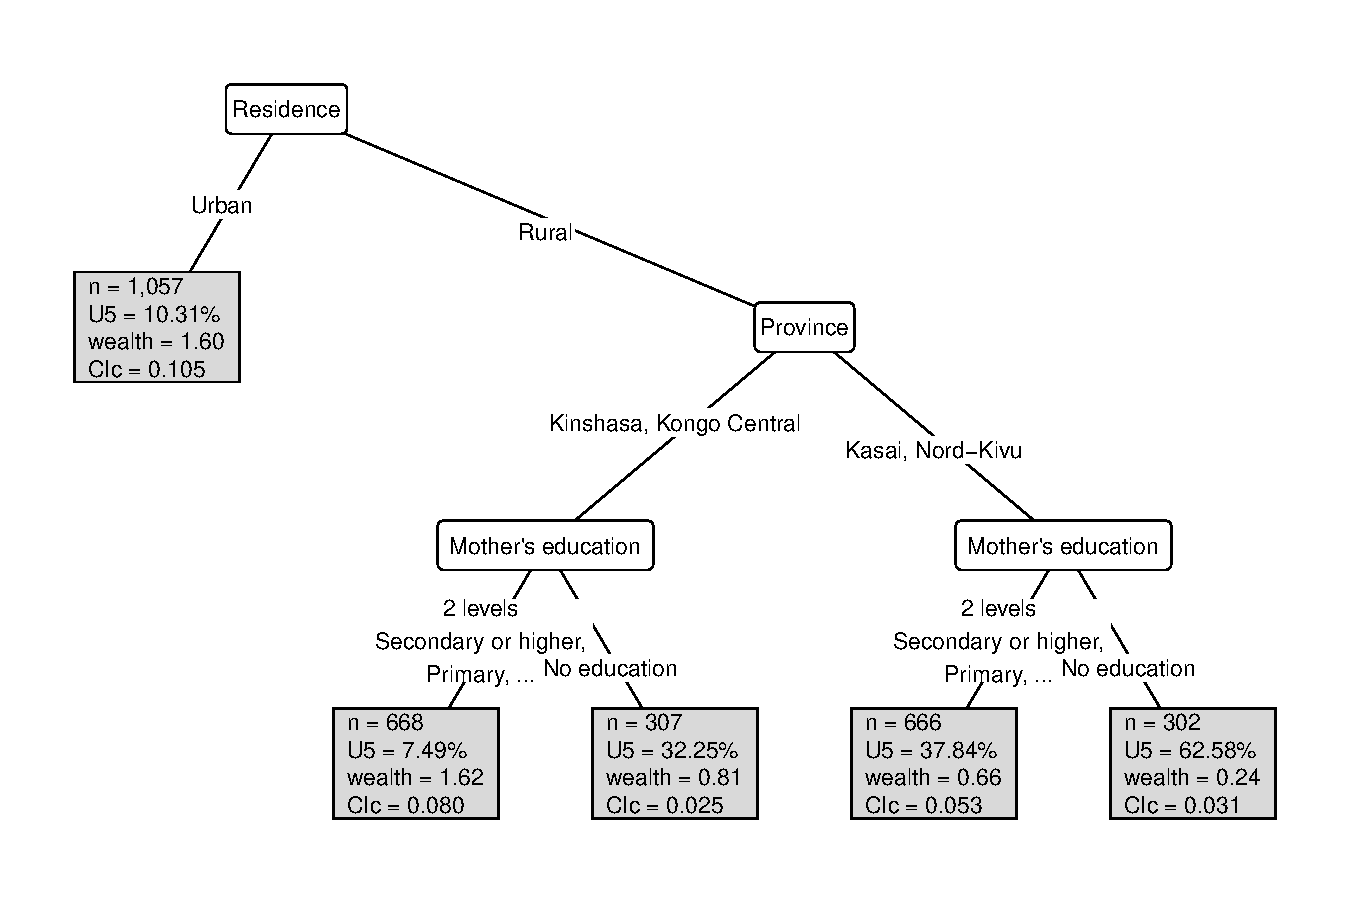
\includegraphics[keepaspectratio]{Decomposition_of_CI_Trees_MM_files/figure-pdf/fig-appendix-simulation-positive-control-cic-1.pdf}}

}

\caption{\label{fig-appendix-simulation-positive-control-cic}Positive-control
simulation tree fitted with the CIc criterion.}

\end{figure}%

\begin{figure}[H]

\centering{

\pandocbounded{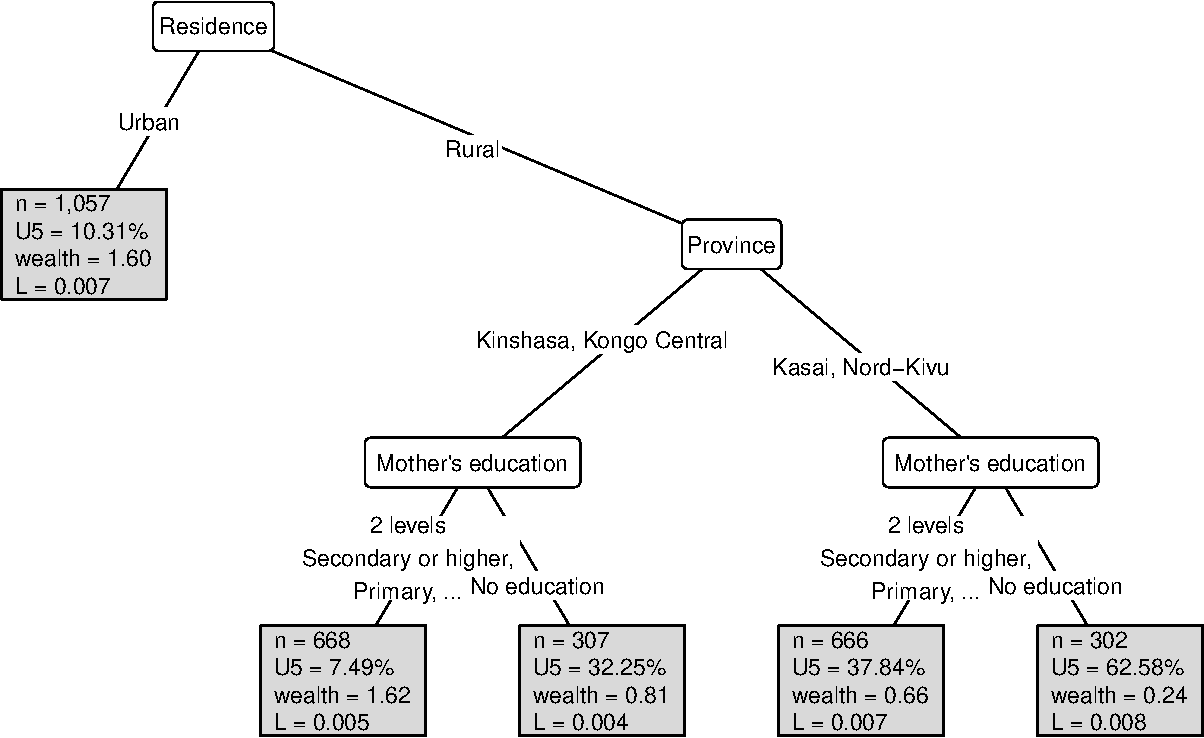
\includegraphics[keepaspectratio]{Decomposition_of_CI_Trees_MM_files/figure-pdf/fig-appendix-simulation-positive-control-l-1.pdf}}

}

\caption{\label{fig-appendix-simulation-positive-control-l}Positive-control
simulation tree fitted with the L criterion.}

\end{figure}%




\end{document}
